\chapter{Structural constitutive models for planar collagenous soft tissues}


\section*{Preface}
\addcontentsline{toc}{section}{Preface}%

    Fundamental to developing a deeper understanding of soft tissue function and pathology is the development of an accurate tissue-level constitutive model. In the present work, we developed a novel meso-scale (i.e. at the level of the fiber, 10-100 $\mu$m in length scale) structural constitutive model (MSSCM) with application to MV leaflet. This model takes into account the layered structure of these tissue and the contributions from the distinct collagen and elastin fiber networks within each tissue layer. Requisite collagen and elastin fibrous structural information for each layer were quantified using second harmonic generation microscopy and conventional histology. A comprehensive mechanical data set was also used to guide model formulation and parameter estimation. Furthermore, novel to tissue-level structural constitutive modeling approaches, we allowed the collagen fiber recruitment function to vary with orientation. Finally, a novel fibril-level (0.1 to 1 $\mu$m) validation approach was used to compare the predicted collagen fiber/fibril mechanical behavior with extant MV small angle X-ray scattering data. Results demonstrated excellent agreement, indicating that the MSSCM fully captures the tissue-level function. Future utilization of the MSSCM in computational models of the MV will aid in producing highly accurate simulations in non-physiological loading states that can occur in repair situations, as well as guide the form of simplified models for real-time simulation tools.

\textbf{The work contained in this chapter was published as}:  Zhang, W.; Ayoub, S.; Liao, J. \& Sacks, M. S.
A meso-scale layer-specific structural constitutive model of the mitral heart valve leaflets 
Acta Biomater, 2016, 32, 238-55 


%---    INTRODUCTION
\section{Introduction}
    
    The mitral valve (MV) is the most structurally complex and physically demanded valve within the heart. It is one of the most suitable choices for the development and validation of a generalized meso-scale structural constitutive model (MSSCM). According the American Heart Association in 2013, it is estimated that MV disease is present in over 4 million adults \cite{go_heart_2014}. MV regurgitation is the most common pathology resulting from myocardial infarction (ischemic mitral regurgitation or IMR). The most frequent corrective approach used to restore leaflet function is MV annuloplasty \cite{kaneko_mitral_2014, amini_vivo_2012}, wherein an annuloplasty ring is used to induce MV leaflet closure during systole. However, such procedures alter the distribution of stress within the leaflet \cite{amini_vivo_2012,salgo_effect_2002,mahmood_three_2009,jimenez_saddle_2007,padala_saddle_2009,sacks_vivo_2006,eckert_vivo_2009,rausch_vivo_2011}, which may influence the long-term durability of the repair procedure. Long-term studies suggests that 60\% of patients who underwent MV repair show recurrence of MV regurgitation within 3–5 years, and 10–15\% of patients require re-operation within the following 10 years \cite{flameng_recurrence_2003,flameng_durability_2008}. The need for computational models, based on understanding of the underlying mechanobiological processes is self-evident for predicting the outcome of surgically repaired MVs and driving the development of improved patient-specific surgical techniques.
    
    
    While MV leaflets may first appear essentially to be membranous flaps, they are in actuality complex multilayered structures that undergo large anisotropic deformations in vivo \cite{sacks_vivo_2006}. Specifically, there are four morphologically distinct layers of the MV: the ventricularis, fibrosa, spongiosa, and atrialis \cite{carruthers_alterations_2012}. All layers are composed of various amounts of dense networks of collagen (mostly type I) and elastin fibers, as well as non-fibrous proteoglycans (PG) and glycosaminoglycans (GAG). In a recent study \cite{lee_quantification_2015}, we demonstrated that the layer-specific deformations of the MV interstitial cells (MVIC) are a direct result of the layer-specific architectures. This suggests that layer-specific adaptations are possible, as observed in Wells et al.\cite{wells_physiological_2012}. Yet, it remains unclear as to (1) why the MV has this distinct pattern of layers, (2) what the respective mechanical roles of each layer are, and (3) how does these patterns relate to the bulk macro-scale responses.
    
    
    The underlying layer-specific differences in mechanical properties are a result from the constituent fiber populations. Type I collagen is the most abundant protein found in MV tissue, and it is the major determinant of its mechanical behavior \cite{parry_molecular_1988,gelse_collagens_2003}. The functional subunit of collagen is the collagen fibril, which composed of tropocollagen molecules that arrange themselves into a quarter stacking array \cite{parry_molecular_1988,gelse_collagens_2003}. It is this structure that allows small angle X-ray scattering (SAXS) studies to measure the underlying fibril deformations for tendon \cite{sasaki_elongation_1996,sasaki_stress_1996} and MV leaflet tissues \cite{liao_relation_2007}. At the next structural level, the collagen fibrils group to form collagen fibers. There is an incomplete understanding regarding the functional relationship between collagen fibers and the fibrils. In fact, the exact definition of collagen fibers in relation to fibrils is usually tissue specific. Like the fibrils from which their functional properties are derived, collagen fibers exhibit tensile strength of up to 1 GPa \cite{shen_stress_2008,gentleman_mechanical_2003,eppell_nano_2006,yang_mechanical_2008,sacks_biomechanics_2009} with low flexural stiffness \cite{sacks_biomechanics_2009}. As a result, collagen fibers typically extend by no more than a 4–5\%. To increase the tissue-level compliance, collagen fibers at the macroscopic scale become sinusoidally crimped \cite{parry_molecular_1988} and does not contribute mechanically until fully straightened. Moreover, the distribution of collagen fiber-level straightening strains is the mechanism for tissue-level non-linearity \cite{lanir_constitutive_1983,sacks_multiaxial_2003}. 
    
    
    In contrast to collagen, elastin forms complex cross-linked fibrous networks with comparatively low modulus that are thought to assist in tissue recoil \cite{debelle_elastin_1999,debelle_structures_1999} and maintaining collagen fiber crimp \cite{vesely_comparison_1998,scott_aortic_1995}. Unlike large arteries, elastin is present in much lower quantities in valvular tissues compared to collagen \cite{sacks_biomechanics_2009,vesely_comparison_1998,lis_biochemical_1987,stella_biaxial_2007} and its role in valve mechanics is not well understood. Finally, we note that glycosaminoglycans (GAGs) are known to affect water retention and hysteresis in valvular tissues \cite{lovekamp_stability_2006,eckert_biomechanical_2013}, with the loss of GAGs known to reduce cuspal thickness and diminish rehydration capacity. However, GAGs are not a primary load bearing component, but appear act as a dampening mechanism to smooth rapid bending motions of the leaflet during valve function \cite{eckert_biomechanical_2013}.
    
    
    Thus, a more complete understanding of MV function and failure must involve an improved understanding of how the above MV leaflet structures mechanically interact. This is best done through the mathematical development of constitutive models that incorporate these features, which can aid both in providing insight and in forming a predictive modeling framework for their remodeling and failure. In the present, work we developed a novel comprehensive meso-scale (i.e. at the level of the fiber) structural constitutive model (MSSCM) for MV leaflets, focusing on the specific collagen and elastin fiber networks within each of its four distinct layers. We used a comprehensive set of structural and mechanical studies (Table \ref{c2tab:experiments}) and a rigorous experimentally guided approach to tackle model formulation, parameter optimization and model validation (Fig. 1). The results were then validated at both the micro (fibril) and tissue-level using a novel approach based on a previous SAXS study on the mitral valve \cite{liao_relation_2007}, and again at the meso-scale using measured fiber structures. We also explored a novel extension to previous structural constitutive model approaches \cite{hollander_constitutive_2011,chen_micromechanics_2011,fata_insights_2014,sacks_incorporation_2003} to allow for angular dependency of collagen fiber recruitment (orientation-variant) and assessed the model predictive capabilities under extra physiological loading that could occur in post-surgical scenarios.
    
\begin{table}\label{c2tab:experiments}
\centering
\caption{Experimental Techniques and Deliverables}
 \begin{tabular}{|m{.2in}|L{0.6in}|L{1in}|L{2.5in}|L{0.95in}|}
 \hline
 &  \textbf{Study}  & \textbf{Description}  & \textbf{Purpose}  & \textbf{Description}  \\
 \hline
 
 \multirow{2}{0.2in}{\rotatebox[origin=c]{90}{Structural}}
 & SHG  
 & Image of fluorescently labeled collagen and elastin 
 & Image processing is done to quantify the fiber orientation distribution function of collagen and elastin within each layer. 
 & ODF (used for validation) \\
 \cline{2-5}
 
 & Histology
 & Collagen, elastin and Proteoglycans are stained in a transmural slice. 
 & The image is separated into channels and is used to quantify the mass fractions and relative fraction of collagen and elastin of each layer. This is used directly in the model. 
 & Mass fractions   \\
 \hline
 
 \multirow{1}{0.2in}{\rotatebox[origin=c]{90}{Mechanical}}
 & SAXS
 & X-ray scattering at a length comparable to D-period of the fiber
 & The SAXS scatter pattern have periods related to the D-period of the collagen fibers. The D-period can be used to quantify the fiber-level strain and the fiber stiffness
 & Collagen Fiber Modulus, (for validation)   \\
 \cline{2-5}
 
 & Planar Biax (EB)
 & Biax with equal strain along both axes
 & Under equibiaxial strain, we can recover the ensemble stress from the sum of the axial stresses. This allows us to model the ensemble stress directly to determine the fiber modulus and fiber recruitment.
 & \multirow{1}{0.95in}{Collagen Fiber Modulus, Recruitment Parameters (For validation)}  \\
 \cline{2-4}
 
 & Uniaxial	
 & Tissue is deformed along the preferred direction of the fibers
 & With the tight splay, under uniaxial extension all fibers become nearly aligned to the test axis, allowing us to use a simplified model rather like using the ensemble stress to recover the fiber modulus and recruitment. 	& \\
 \cline{2-5}
 
 & Planar Biax (Multi-prot)	
 & Data is taken over the physiological and extra-physiological range.	
 & This with us the data to performed parameter estimation to determine the properties of the MV. The outer extra-physiological protocols can be used check the predictive ability of the model. 
 & Layer dependent material properties.     \\
 \hline
 
 \end{tabular}
\end{table}

%---    METHODS
\section{Methods}

\subsection{General consideration and assumptions}\label{sec:generalconsiderations}

\subsubsection{Collagen fibrils and fibers} \label{sec:collagenconsiderations}

    In the present work, we assumed that the collagen fibrils were contiguous subunits of the collagen fibers, so that there was negligible slippage between fibrils. To characterize the straightening behavior of the fiber-level crimped structure \cite{lanir_constitutive_1983, fata_insights_2014, sacks_incorporation_2003, lanir_structural_1979, kastelic_structural_1980, hansen_recruitment_2002, cacho_constitutive_2007, grytz_constitutive_2009}, we use only the fiber axial stretch needed to fully straighten the fiber, slack stretch, rather than the period and amplitude of the collagen fibers. This avoids the necessity of incorporating detailed unloaded geometry for the collagen fibers.


    In most structural models, the distribution of collagen slack strains (the recruitment distribution) is assumed to be independent of the orientation. This approach has the advantage of allowing collagen fiber recruitment model parameters to be determined directly from a single planar equibiaxial strain (EB) tests, where the deformation gradient tensor is $F = \operatorname{diag}[\lambda, \lambda, 1/\lambda^2$] and no fiber rotations occur (e.g. \cite{fata_insights_2014}). For bovine pericardium, we have shown that when the collagen fiber orientation distribution function (ODF) is obtained independently, the complete in-plane response can be predicted \cite{sacks_incorporation_2003}. However, some angular dependence may be physiologically relevant for general tissues. For example, collagen fibers are constantly produced and degraded under physiological stresses, and generally prefer to function within homeostatic stress levels \cite{humphrey_cardiovascular_2002}. Moreover, MV leaflets experience large and highly anisotropic deformations in vivo, which would induce substantially higher fiber ensemble stresses in the larger strain direction \cite{amini_vivo_2012,sacks_vivo_2006}. We thus speculate that collagen fibers may exhibit larger undulations in the directions of larger physiological strain to maintain a constant fiber ensemble stress. However, the exact dependence of collagen recruitment on fiber orientation remains unknown and has yet to be explored in the literature.
    
    
    For the collagen fiber material model, a stress–strain relation that is linear in 2nd Piola Kirchhoff stress and Green Lagrange strain is the predominant fiber model of choice [40], [41], [47]. However, SAXS studies of intact tissue shows that the fibril strain varies linearly with applied forces in tendon [18], [19] and MV leaflet tissues [20], [21]. Furthermore, the results are corroborated by the atomistic modeling results by Buehler [48], where the force displacement relation is essentially linear at strains lower than 0.35.
    
    
    For the collagen fiber material model, a stress–strain relation that is linear in 2nd Piola Kirchhoff stress and Green Lagrange strain is the predominant fiber model of choice \cite{sacks_incorporation_2003,lanir_structural_1979,fan_simulation_2014}. However, SAXS studies of intact tissue shows that the fibril strain varies linearly with applied forces in tendon \cite{sasaki_elongation_1996,sasaki_stress_1996} and MV leaflet tissues \cite{liao_relation_2007}. Furthermore, the results are corroborated by the atomistic modeling results by Buehler \cite{buehler_atomistic_2006}, where the force displacement relation is essentially linear at strains lower than 0.35.
    



\subsubsection{Elastin fiber network} \label{sec:elastinconsiderations}

    Elastin fibers function through an entropy-driven process wherein the decrease in entropy drives the increase in fiber stress as the fiber is elongated. As of yet, there is no first-principle form for elastin when modeled either as a continuous phase or a discrete fibrous network. Typical MV models are either purely phenomenological or ignore the elastin component entirely. In a previous study on ovine pulmonary artery \cite{fata_insights_2014}, we found the elastin fibers to behave linearly in second Piola–Kirchhoff stress and Green Lagrange strain. However, the specific form of the elastin likely depends on a variety of factors including cross-linking and residual strain. Moreover, it is not clear if there are layer-specific differences, and thus a more general material model for the MV elastin fiber network is needed.




\subsubsection{Affine kinematics and layer averaged responses}

    As in previous structural approaches, we assume affine fiber kinematics. This assumption is supported by a recent study wherein we demonstrated that the MV anterior leaflet collagen and elastin fibers all deformed in a manner consistent with affine deformation kinematics \cite{lee_presence_2015}. We further assume each layer is structurally homogeneous (i.e. ignore intra-layer structural variations). Thus, and in order to derive the total individual layer response as a function of its collagen and elastin components, the following information was used (Table \ref{c2tab:experiments}):
        \begin{enumerate}
            \item The mass composition of each layer, including the quantities of collagen and elastin.
            \item The ODF for the collagen and elastin fibers within each layer.
            \item The recruitment behaviors of the collagen fiber network for each layer.
        \end{enumerate}
    Finally, the following assumptions were made according to the current understanding of heart valve leaflet tissues:
        \begin{enumerate}
            \item All layers are tightly bonded with no slippage, similar to what is observed in the aortic valve leaflet \cite{buchanan_interlayer_2013}.
            \item There are no mechanical interactions between layers and that they deform with the bulk tissue.
            \item The collagen fiber modulus is the same for all layers and that the differences in collagen mechanical contribution response are due to variations in structural organization.
            \item Fiber–fiber interactions are negligible.
            \item Fiber–matrix interactions are negligible.
        \end{enumerate}




%%%%%%%%%%%%%%%%%%%%%%%%%%%%%%%%%%%%%%%%
\subsection{Constitutive model formulation}

\subsubsection{Single fiber models}

    Based on the above considerations (Section \ref{sec:collagenconsiderations}), the following linear force displacement relation for the collagen fibrils and fibers was used
        %-------------------	begin EQUATION 	-------------------%
        \begin{equation}\label{eqn:collagenfiberlaw}
        \begin{aligned}
        P_f =& \eta_{C}\left(\lambda_t - 1\right)\frac{1}{\lambda_s} = \frac{\eta_C}{\lambda_s}\left(\frac{\lambda_f}{\lambda_s} - 1\right)    \\
        S_f =& \frac{1}{\sqrt{2E_s + 1}}\left( \frac{1}{\sqrt{2 E_s + 1}} - \frac{1}{\sqrt{\sqrt{2E_f + 1}}}\right)
        \end{aligned}
        \end{equation}
        %-------------------	 end EQUATION 	-------------------%
    where $P_f$ and $S_f$ are the 1st and 2nd Piola Kirchhoff fibers stresses, $\eta_C$ is the collagen fiber modulus, $\lambda_f$ and $E_f$ are the fiber stretch and Green’s strain, $\lambda_t$ and $E_t$ are the true fiber stretches and Green’s strains, and $\lambda_s$ and $E_s$ are the slack fiber stretches and Green’s strains. For the elastin fibers, based on Section \ref{sec:elastinconsiderations} and our previous work on the pulmonary artery \cite{fata_insights_2014}, we use the following generalized form,
        %-------------------	begin EQUATION 	-------------------%
        \begin{equation}\label{eqn:elastinfiberlaw}
        \begin{aligned}
        S^e_f = \eta_e \left( E^e_f\right)^d
        \end{aligned}
        \end{equation}
        %-------------------	 end EQUATION 	-------------------%
    Here $\eta_e$ is the elastin fiber modulus and $d$ is the exponent that determines the degree of non-linearity of the fiber. This allows us to alter the stress strain relationship of the fiber based on the mechanical and structural data acquired.




\subsubsection{Fiber ensemble models}

    As in previous works \cite{lanir_constitutive_1983,sacks_incorporation_2003,fan_simulation_2014}, we scale up to the tissue-level by first considering an ensemble of collagen fibers, which is defined as a sub-group of fibers that share a common initial orientation $n_0$. Collagen fiber recruitment is commonly assumed to be independent of $n_0$, i.e. is orientation-invariant \cite{fata_insights_2014,sacks_incorporation_2003,lanir_structural_1979,fan_simulation_2014}. To evaluate the hypothesis that there may be angular variations is due to homeostasis (Section \ref{sec:collagenconsiderations}), we developed the following generalized framework for orientation-variant fiber recruitment. The fiber recruitment distribution function $D\left[E_s(n_0)\right]$ is a function of the fiber slack strain $E_s$ and orientation $n_0$, and is represented by a beta distribution function. $D\left[E_s(n_0)\right]$ was parametrized by a mean $\mu_r$, a standard deviation $\sigma_r$, and was defined over a strain range bounded by the lower- and upper-bounds $E_{lb}$ and $E_{ub}$. The general form given by,
        %-------------------	begin EQUATION 	-------------------%
        \begin{equation}\label{eqn:recruitmentdistribution}
        \begin{aligned}
        D(\mathbf{\xi},E_s) = \frac{(y)^{\alpha-1}(1-y)^{\beta-1}}{B(\alpha,\beta)(E_{ub}-E_{lb})}, 
            \quad y = \frac{E_s - E_{lb}}{E_{ub} - E_{lb}}, \quad y \in (0,1)
        \end{aligned}
        \end{equation}
        %-------------------	 end EQUATION 	-------------------%
    where the parameter vector is $\mathbf{\xi} = \{\mu, \sigma, E_{lb}, E_{ub} \}$. Here, $B(\alpha, \beta)$ is the Beta distribution function with shape parameters $\alpha$, $\beta$. The interrelationships between the two are
        %-------------------	begin EQUATION 	-------------------%
        \begin{equation}\label{eqn:recruitmentparameters}
        \begin{gathered}
        \hat{\mu}_r = (\mu_r - E_{lb})/(E_{ub} - E_{lb}), \quad \hat{\sigma}_r = \sigma_r/(E_{ub} - E_{lb}),  \\
        \alpha = \frac{-\hat{\mu}_r (\hat{\sigma}_r^2 + \hat{\mu}_r^2 - \hat{\mu}_r)}{\hat{\sigma}_r^2}, \quad \beta = \frac{(\hat{\mu}_r - 1) (\hat{\sigma}_r^2 + \hat{\mu}_r^2 - \hat{\mu}_r)}{\hat{\sigma}_r^2}, \\
        \mu_r \in (E_{lb}, E_{ub}), \quad \Hat{\mu}_r \in (0,1)
        \end{gathered}
        \end{equation}
        %-------------------	 end EQUATION 	-------------------%
    It should be noted that the parameters in Eqns \ref{eqn:recruitmentdistribution}, \ref{eqn:recruitmentparameters} are functions of the initial fiber ensemble orientation $n_0$, so that $\xi (n0)$.


    While comprehensive, equations \ref{eqn:recruitmentdistribution}, \ref{eqn:recruitmentparameters} present difficulties in actual implementation by either direct experimental measurement or parameter estimation \cite{hill_theoretical_2012}. However, the equations can be reduced using the assumption that the ensemble stresses are constant with orientation. Here the ensemble strain Es is scaled by the maximum ensemble strain $E_{max}(\mathbf{n}_0)$ in the fully loaded state.
        %-------------------	begin EQUATION 	-------------------%
        \begin{equation}\label{eqn:recruitmentasafunctionofangle}
        \begin{aligned}
        D(\mathbf{\xi},E_s) = \bar{D}\left(\bar{\mathbf{\xi}}, \frac{E_s}{E_max(\mathbf{n}_0)}\right)
        \end{aligned}
        \end{equation}
        %-------------------	 end EQUATION 	-------------------%
    where the parameter vector is now $\bar{\mathbf{\xi}} = \bar{\mathbf{\xi}}(\mathbf{n}_0) = (\bar{\mu}, \bar{\sigma}, \bar{E}_{lb}, \bar{E}_{ub})$, which is non-dimensionalized as indicated by the overbar. Using this form, the same fraction of fibers is recruited for each fiber ensemble at the maximum strain and the ensemble stresses becomes approximately constant with orientation. This form also requires no additional parameters. In addition to the above analysis, we utilized the standard orientation-invariant approach \cite{fata_insights_2014} defined as
        %-------------------	begin EQUATION 	-------------------%
        \begin{equation}\label{eqn:recruitmentasafunctionnormal}
        \begin{aligned}
        D(\mathbf{\xi},E_s) = D(\{\mu_r, \sigma_r, E_{lb}, E_{ub}\}, E_s(\mathbf{n}_0))
        \end{aligned}
        \end{equation}
        %-------------------	 end EQUATION 	-------------------%
    For both forms, the resulting ensemble stress is given by
        %-------------------	begin EQUATION 	-------------------%
        \begin{equation}\label{eqn:collagenensemblestress}
        \begin{aligned}
        &S_e^{ens}\left[ \mathbf{\xi}, E_{ens}(\mathbf{n}_0)\right] = 
            \eta_C \int_0^{E_{ens}(\mathbf{n}_0)} \frac{D(\xi,x)}{\sqrt{2x+1}} 
                \left(\frac{1}{\sqrt{2x+1}} - \frac{1}{\sqrt{2E_{ens}(\mathbf{n}_0)+1}}\right)  \\
        &\mathrm{where} \quad D(\mathbf{\xi}, x) = 
            \begin{cases} 
                \bar{D}(\bar{\mathbf{\xi}},x,\mathbf{n}_0) & \text{orientation variant} \\
                D(\mathbf{\xi},x) & \text{orientation invariant} 
            \end{cases}
        \end{aligned}
        \end{equation}
        %-------------------	 end EQUATION 	-------------------%
    Finally, since elastin fibers are straight (i.e. not undulated like collagen fibers), the elastin ensemble stress is simply $S_e^{ens} = \eta_e(E_{ens})^d$.
    



\subsubsection{Complete layer and full tissue forms}

    The strain energy of collagen and elastin fibers for each layer is given by the sum of the fiber ensembles weighted by the fiber ODF $\Gamma(\theta)$ and mass fraction with respect to each layer $\phi$. $\Gamma(\theta)$ is approximated using another beta distribution function with a mean $\mu$ and standard deviation $\sigma$ \cite{fata_insights_2014}. Since $\Gamma(\theta)$ is nearly symmetric, the shape parameters $\alpha$ and $\beta$ are forced to be equal (Eqn. \ref{eqn:recruitmentparameters}), thus $\bar{\mu} = 0.5$ at all points. A remainder function is then used to ensure $\theta \in \left[\mu - \pi/2, \mu + \pi/2 \right]$, before normalizing it to the domain of the beta function $y \in \left[0,1\right]$, yielding
        %-------------------	begin EQUATION 	-------------------%
        \begin{equation}\label{eqn:orientatinodistributionfunction}
        \begin{aligned}
        \Gamma(\theta) = \frac{B(\alpha,\alpha,y)}{\pi}, \quad y = \frac{\operatorname{Mod}(\theta - (\mu -     \pi/2), \pi)}{\pi}, \\
        \alpha = -0.5 \left(\bar{\sigma}^2 + 0.25 -0.5\right)/\bar{\sigma}^2, \quad \bar{\sigma} = \sigma/\sigma\pi
        \end{aligned}
        \end{equation}
        %-------------------	 end EQUATION 	-------------------%
    where $B$ is the Beta function.
    
    
    Next, we define the tissue “matrix” as PG, GAGs, and water into a homogenized single phase and represented using an incompressible Neo–Hookean model. The resulting matrix stress tensor, assuming a planar configuration and no distinctions between layers, is $S_m = \mu_m(\mathbf{I} - C_{33}\mathbf{C}^{-1})$. This phase is necessary to enforce incompressibility and to obtain accurate results in computational simulations \cite{fan_simulation_2014}. The resulting total tissue stress, weighted by the mass fractions $\phi$, is given by
        %-------------------	begin EQUATION 	-------------------%
        \begin{equation}\label{eqn:multilayeredstressform}
        \begin{aligned}
        \mathbf{S} =& \sum_{L = 1}^\mathrm{n layers} \left\{
        \begin{array}{l}
        \phi_c^L\eta_c\int_{-\pi/2}^{\pi/2}\Gamma_c^L(\theta)\int_0^{E_{ens}(\theta)} \frac{D_L(x,\theta)}{\sqrt{2x+1}}\left( \frac{1}{\sqrt{2x+1}} - \frac{1}{\sqrt{2E_{ens}(\theta)+1}} \right) \mathbf{n}_0\otimes\mathbf{n}_0 \dif x\dif\theta\\
        + \phi_e^L\eta_e^L\int_{-\pi/2}^{\pi/2}\Gamma_e^L(\theta)(E_{ens})^{d_L} \mathbf{n}_0\otimes\mathbf{n}_0 \dif\theta
        \end{array}
        \right\}    \\
        &+ \phi_m\eta_m\left(\mathbf{I} - C_{33}\mathbf{C}^{-1}\right)
        \end{aligned}
        \end{equation}
        %-------------------	 end EQUATION 	-------------------%
    where the superscript L indicates the layer and the parameter list for Eqn. \ref{eqn:multilayeredstressform} is given in Table \ref{c2tab:modelparameters}.


\begin{table}
\centering
\caption{Experimental Techniques and Deliverables}\label{c2tab:modelparameters}
\begin{tabular}{L{.15in}L{0.2in}C{0.3in}L{2.8in}L{1.0in}}
\hline
& \multicolumn{2}{c}{\textbf{Parameter}}
& \textbf{Description}  
& \textbf{Layer}   \\
\hline

\multirow{12}{*}{\rotatebox[origin=c]{90}{Collagen}}
& 1    & $\eta_c$  & Mean collagen fiber modulus   &  \\
\cline{2-5}
& 2    & $\sigma_c^f$   & \multirow{2}{2.7in}{Standard Deviation of the collagen fiber ODF}  & Fibrosa   \\
& 3    & $\sigma_c^a$   &   & Atrialis  \\
\cline{2-5}
& 4    & $\mu_c^f$      & \multirow{3}{2.7in}{Mean of the collagen fiber recruitment distribution} & Fibrosa    \\
& 5    & $\mu_c^a$      &   & Atrialis    \\
& 6    & $\mu_c^s$      &   & Spongiosa    \\
\cline{2-5}
& 7    & $\sigma_r^f$   & \multirow{3}{2.7in}{Standard deviation of the collagen fiber recruitment distribution} & Fibrosa    \\
& 8    & $\sigma_r^a$   &   & Atrialis    \\
& 9    & $\sigma_r^s$   &   & Spongiosa    \\
\cline{2-5}
& 10   & $E_{ub}^f$     & \multirow{3}{2.7in}{The upper-bound of the collagen fiber recruitment distribution} & Fibrosa    \\
& 11   & $E_{ub}^a$     &   & Atrialis    \\
& 12   & $E_{ub}^s$     &   & Spongiosa    \\
\cline{2-5}
\hline

\multirow{8}{*}{\rotatebox[origin=c]{90}{Elastin}}
& 13    & $\sigma_e^v$   & \multirow{2}{2.7in}{Standard deviation of the elastin fiber ODF}  & Ventricularis   \\
& 14    & $\sigma_e^a$   &   & Atrialis  \\
\cline{2-5}
& 15    & $\eta_e^f$      & \multirow{3}{2.7in}{Mean elastin ensemble modulus} & Ventricularis    \\
& 16    & $\eta_e^a$      &   & Atrialis    \\
& 17    & $\eta_e^s$      &   & Spongiosa    \\
\cline{2-5}
& 18    & $d_e^f$      & \multirow{3}{2.7in}{Mean elastin ensemble exponent} & Ventricularis    \\
& 19    & $d_e^a$      &   & Atrialis    \\
& 20    & $d_e^s$      &   & Spongiosa    \\
\hline

\multirow{2}{*}{\rotatebox[origin=c]{90}{Matr.}}
& 21    & $\eta_m$  & Mean matrix shear modulus	homogenized over all four layers   &  \\
& 22    & $\mu_\theta$  & Preferred direction of the mitral valve leaflet relative to the testing axes		   &  \\
\hline
\end{tabular}
\end{table}







%%%%%%%%%%%%%%%%%%%%%%%%%%%%%%%%%%%%%%%%
\subsection{Structural characterization} \label{c2sec:structure}

    To obtain the mass fractions of the major ECM components for each layer, additional porcine MV leaflets (n = 3) were harvested from a local slaughter house and immediately transported for sectioning. Transverse sections from the central region of each leaflet were stained using Movat’s Pentachrome stain (Fig. \ref{c2:fig:2}), and then imaged using light microscopy to determine the relative thickness of each layer. Color deconvolution was then used to separate the collagen (yellow), elastin (Black), and PGs (Blue). The relative area fraction in each layer was determined using the total color intensity (Table \ref{c2tab:massfractions}). ODFs for both collagen and elastin fiber networks were quantified by SHG imaging using methods described by Carruthers et al. \cite{carruthers_alterations_2012} (Fig. \ref{c2:fig:2}). The resulting orientation distribution functions (ODF) for collagen and elastin were obtained using the methods of Courtney et al. \cite{courtney_design_2006}.
    
    


%%%%%%%%%%%%%%%%%%%%	begin FIGURE 	%%%%%%%%%%%%%%%%%%%%
\begin{figure}
\centering
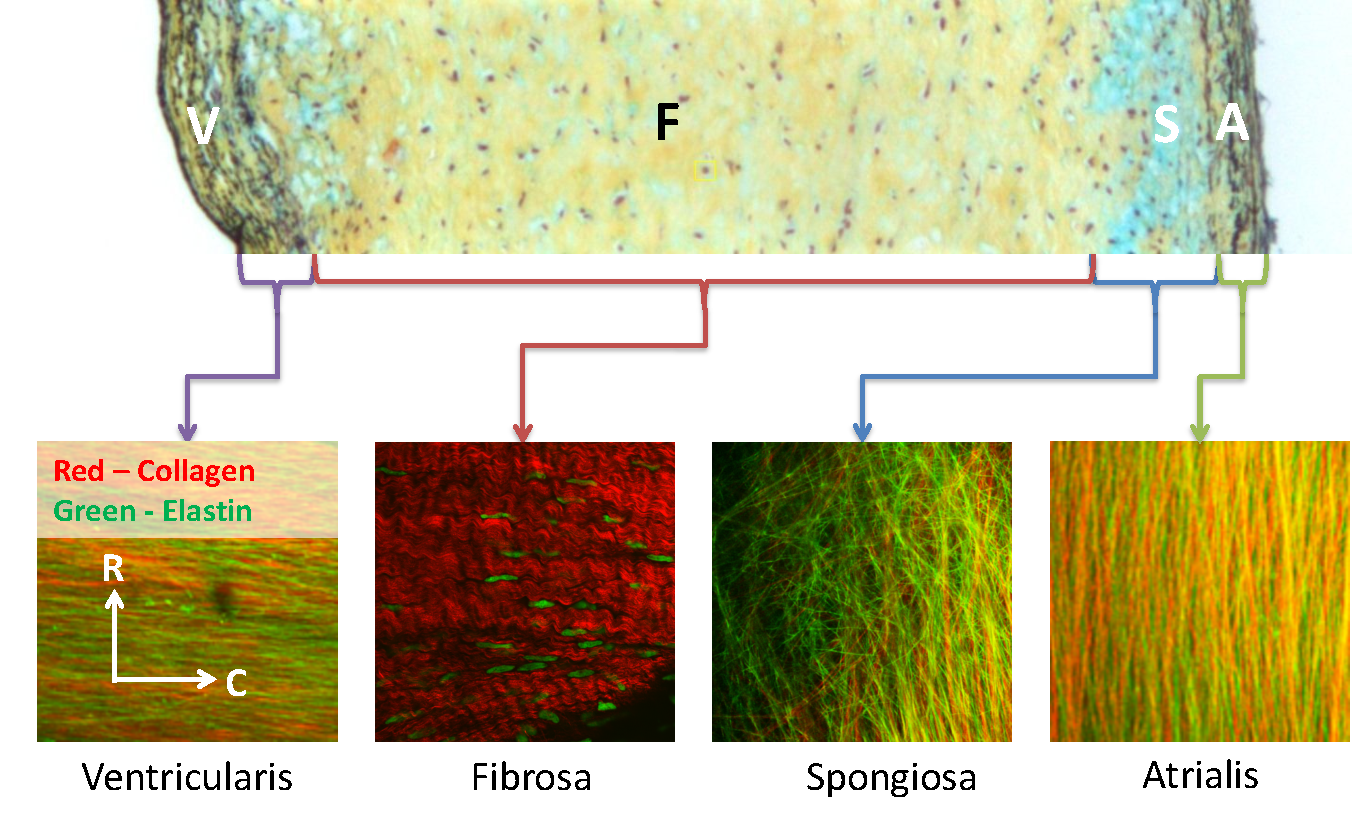
\includegraphics[width=\textwidth]{Images/chapter2/figure2.pdf}
\caption{Microstructural analysis was done using Movat pentachrome stain of the transverse-radial section of the center region of the MV anterior leaflet (Top), and multiphoton microscopy (MPM) of the ventricularis (V), fibrosa (F), spongiosa (S) and atrialis (A) layer of the anterior leaflet (Bottom). The histological section shows the relative thickness of each layer, and the MPM shows the orientation or collagen (red) and elastin (green) fibers in each layer.}
\label{c2:fig:2}
\end{figure}
%%%%%%%%%%%%%%%%%%%%	 end FIGURE 	%%%%%%%%%%%%%%%%%%%%



    
\begin{table}
\centering
\caption{Volume fractions of ECM components in MV (unitless)}\label{c2tab:massfractions}
\begin{tabular}{L{.65in}L{0.65in}L{1.05in}L{0.875in}L{0.875in}L{0.875in}}
\hline
\textbf{Leaflet} & \textbf{ECM} & \textbf{Ventricularis} & \textbf{Fibrosa} & \textbf{Spongiosa} & \textbf{Atrialis}   \\
\hline

\multirow{2}{*}{Anterior}
& Collagen  & $0.078\pm0.018$   & $0.839\pm0.021$   & $0.036\pm0.015$   & $0.047\pm0.007$   \\
& Elastin   & $0.487\pm0.039$   & $0.066\pm0.030$   & $0.067\pm0.000$   & $0.380\pm0.036$   \\
\hline
\multirow{2}{*}{Posterior}
& Collagen  & $0.068\pm0.008$   & $0.778\pm0.052$   & $0.043\pm0.018$   & $0.110\pm0.044$   \\
& Elastin   & $0.104\pm0.021$   & $0.067\pm0.017$   & $0.118\pm0.036$   & $0.711\pm0.035$   \\
\hline
\end{tabular}
\end{table}

\subsection{Experimental mechanical studies} \label{c2:sec:mechanicalstudies}

    In order to develop a comprehensive model to simulate the leaflets in both physiological and surgically altered/pathological conditions, it is necessary to explore the MV properties beyond the physiological range. Moreover, no single deformation mode can provide all the data needed for parameter optimization. Thus, the following deformation modes were utilized.


\subsubsection{Uniaxial loading}

    Under uniaxial loading along the circumferential direction, only the highly circumferentially aligned collagen in the fibrosa and ventricularis layers, which constitute the bulk of the MV, are loaded. This aided the preliminary examination of the collagen fibers mechanics, as the contribution of elastin becomes negligible at high stress. To perform these tests, specimens from four anterior MV leaflets were tested under uniaxial strain until failure. Each specimen was cut into 5 by 20 mm stripes with the long axis oriented along the preferred direction (circumferential) of the leaflet. The specimens were clamped at both ends of the long axis with a separation of 13.5 mm to serve as the gauge length. The transverse direction was unconfined and allowed to contract laterally. One end of the clamps was then displaced at a rate of 0.1 mm/s. The tests were manually aborted after the tissue tears. No preconditioning was done and the tissue was not preloaded. To measure the internal strains more accurately, an optical marker tracking method was used \cite{billiar_biaxial_2000}. All testing was done at room temperature in phosphate buffered saline (PBS).


\subsubsection{Equibiaxial planar strain tests}

    EB planar strain kinematics has several important advantages for examining the effective stress–strain relations in MV leaflet tissues. Firstly, like uniaxial testing, the test can be carried out into the MPa range, exceeding physiological stress levels to insure all collagen fibers are fully recruited. Secondly, as there are no fiber rotations, one can obtain the fiber ensemble response under the assumption of orientation-invariant fiber recruitment \cite{fata_insights_2014,sacks_incorporation_2003,fan_simulation_2014}. This allows direct estimation of the orientation-invariant fiber recruitment function and effective fiber modulus.
    
    
    To obtain the requisite EB strain data, porcine MV specimens were harvested from a local slaughter house and immediately transported for testing. 10 mm by 10 mm sections were taken from the center region of each leaflet and mounted to a custom-built biaxial device \cite{grashow_biaxial_2006,grashow_planar_2006} with the circumferential and radial directions aligned to the device axes. The specimens were immersed in PBS and tested at room temperature. The strain was determined via four fiducial markers glued to the central region of the specimen \cite{billiar_biaxial_2000}. The free-floating state was used as the stress-free reference state, while a preload of 1 g was applied for testing purposes. Starting at 10\% strain, each specimens was tested for ten 30 s cycles with the tenth cycle taken as representative. The maximum strain was then systematically increased until a linear stress–strain region was observed. A total of 7 anterior and 7 posterior porcine MV leaflets were tested.


\subsubsection{Full in-plane responses}

    To obtain the necessary mechanical data for full parameter estimation, a comprehensive set of planar biaxial mechanical data was obtained that encompassed the extra-physiological range. Porcine MV specimens were harvested using a protocol similar to the EB strain testing above. Following mounting, these specimens were first preconditioning for 10 cycles at 90 N/m. The specimens were then unloaded, and the post-preconditioned free-floating state was used as the stress-free references state. Similar to the above, a preload of 1 g was applied for testing purposes. For each loading path, the specimens were loaded to a maximum membrane tension of 90 N/m for ten 30 s cycles with the last cycle taken as representative \cite{grashow_biaxial_2006,grashow_planar_2006}. Circumferential ($x_1$) to radial ($x_2$) ratios of $P_{11}:P_{22}$ = 1:2, 3:4, 1:1, 4:3, and 2:1 were used, with two additional extreme loading protocols that represented extra-physiological ranges of 1:10 and 10:1 to evaluate the MSSCM predictive capabilities.
    
    
\subsubsection{Collagen fiber ensemble analysis using SAXS}

    One way we can assess the intrinsic mechanical properties of collagen fibers, dissociated from the effects of crimping, is using fibril-level measurements from SAXS. We thus utilized extant data from a porcine MV study by Liao et al. \cite{liao_relation_2007} to validate the collagen modulus and recruitment. The experiment was performed on MV anterior leaflets specimens, which were loaded under EB stress. SAXS was used at each load step to measure the fibril strain. Experimental details have been provided in \cite{liao_relation_2007}.
    



\subsection{Parameter estimation}

\subsubsection{General considerations}

    Obtaining the true global cost-function minimum can become exceptionally difficult for highly nonlinear models with a large number of parameters, such as equation \ref{eqn:multilayeredstressform}. This will often include issues such as parameter covariance and the presence of local minima. We thus developed the following detailed sequential procedure for parameter estimation using observations from the structure of the MV leaflet (Section \ref{c2sec:structure}).
    
    
    Firstly, the ventricularis is rich in both elastin and collagen, with a relatively narrow ODF and a preferential orientation in the circumferential direction for both fiber types (Fig. \ref{c2:fig:2}). Secondly, the fibrosa, comprising the bulk of the MV leaflet, contains mainly collagen fibers highly aligned to the circumferential direction with almost no elastin except for trace amounts near the spongiosa. Thirdly, the spongiosa contains relatively small amounts of elastin and collagen, both of which are randomly oriented, and is predominately composed of PGs and GAGs. Fourthly, the atrialis contains the largest population of elastin and some collagen, both of which has a narrow ODF and oriented along the radial direction. Fifthly, since the collagen and elastin fibers in the ventricularis and fibrosa were observed to have very similar ODFs, they cannot be separated reliably from a parameter optimization standpoint. Thus, the small amount of elastin in the fibrosa was considered part of the ventricularis elastin, and the collagen in the ventricularis was considered part of the fibrosa collagen. Also, since the collagen and elastin fibers in the ventricularis and fibrosa were found to be identically aligned and orthogonal to the atrialis, their respective preferred directions were fixed during parameter estimation.
    
    
\subsubsection{Modifications for collagen fiber recruitment bounds}

    As observed in both uniaxial and EB strain data (Fig. \ref{c2:fig:3}), a gradual increase in collagen fiber recruitment and a transition to a linear stress–strain response were clearly visible. In preliminary studies of the collagen fiber recruitment probability function $D(E_s)$, we observed that when the lower-bound $E_{lb}$ was sufficiently distant from the mean $\mu_r$, the overall shape of $D(E_s)$ did not change significantly with further decreases in $E_{lb}$. Thus, to reduce the number of parameters, the lower-bound of the distribution was set to $E_{lb} = 0$.
    
    
%%%%%%%%%%%%%%%%%%%%	begin FIGURE 	%%%%%%%%%%%%%%%%%%%%
\begin{figure}
\centering
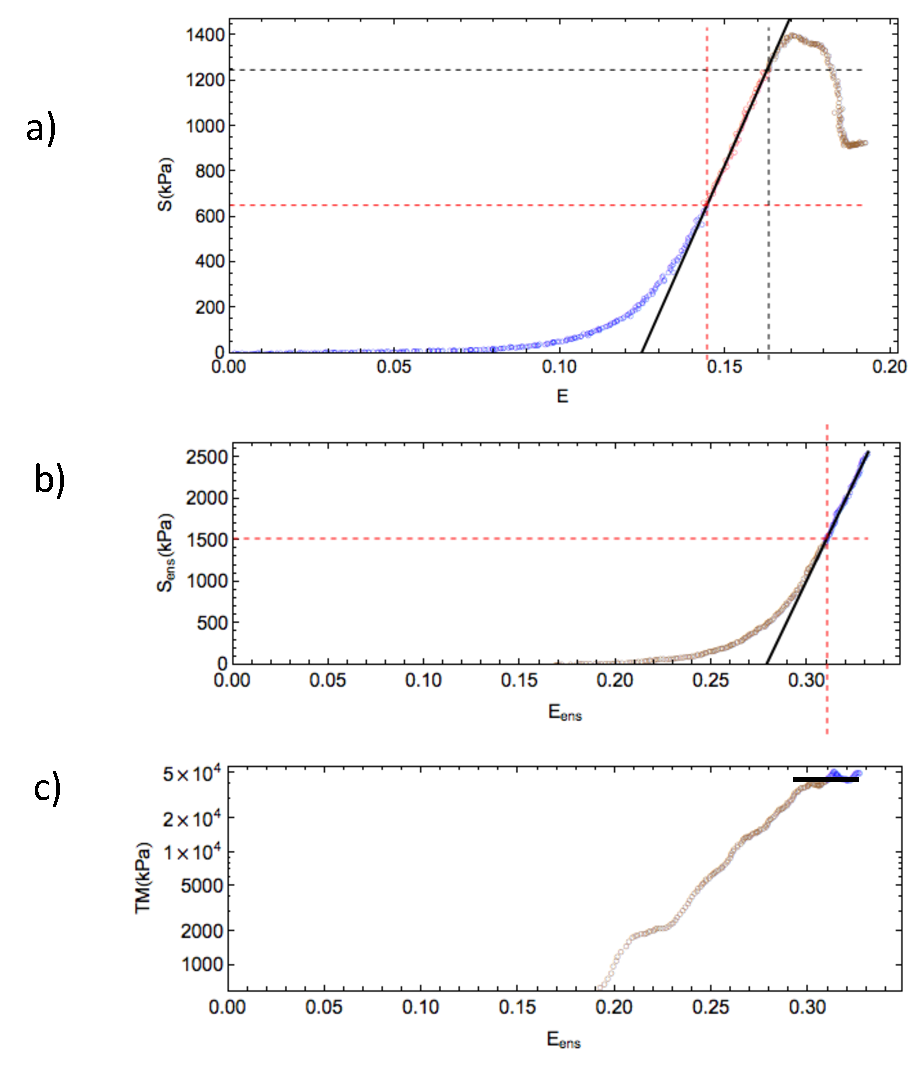
\includegraphics[width=0.95\textwidth]{Images/chapter2/figure3.pdf}
\caption{Example mechanical testing result of (a) uniaxial and (b) and (c) equibiaxial strain test data from an anterior leaflet. The linear post recruitment region is shown by the black line, which indicates full collagen fiber recruitment. The (c) tangent modulus curve in equibiaxial strain test shows a clear flattened section in the post-transition region. Tangent modulus curve for uniaxial extension is not shown due to similarities.}
\label{c2:fig:3}
\end{figure}
%%%%%%%%%%%%%%%%%%%%	 end FIGURE 	%%%%%%%%%%%%%%%%%%%%




\subsubsection{Elastin fiber model} \label{c2:sec:elastinfibermodel}

    To determine the elastin fiber model (Sections \ref{sec:elastinconsiderations} Elastin fiber network, \ref{sec:collagenconsiderations} Single fiber models), we utilized the low stress region of the mechanical response. Due to the collagen fiber recruitment, we can retroactively determine the Elb of the recruitment distribution as the point when the cumulative distribution is less than 1\% (typically less than 3–8 kPa). Since collagen does not contribute significantly in this region, the response in this region can be considered entirely due to elastin (Fig. \ref{c2:fig:4}a). In pilot studies, we found that $d>1$ in equation \ref{eqn:elastinfiberlaw}. In fact, the exponent for the ventricularis and atrialis layer appeared to be different. Thus, we allowed d to vary during parameter estimation rather than being a set to a constant value.


%%%%%%%%%%%%%%%%%%%%	begin FIGURE 	%%%%%%%%%%%%%%%%%%%%
\begin{figure}
\centering
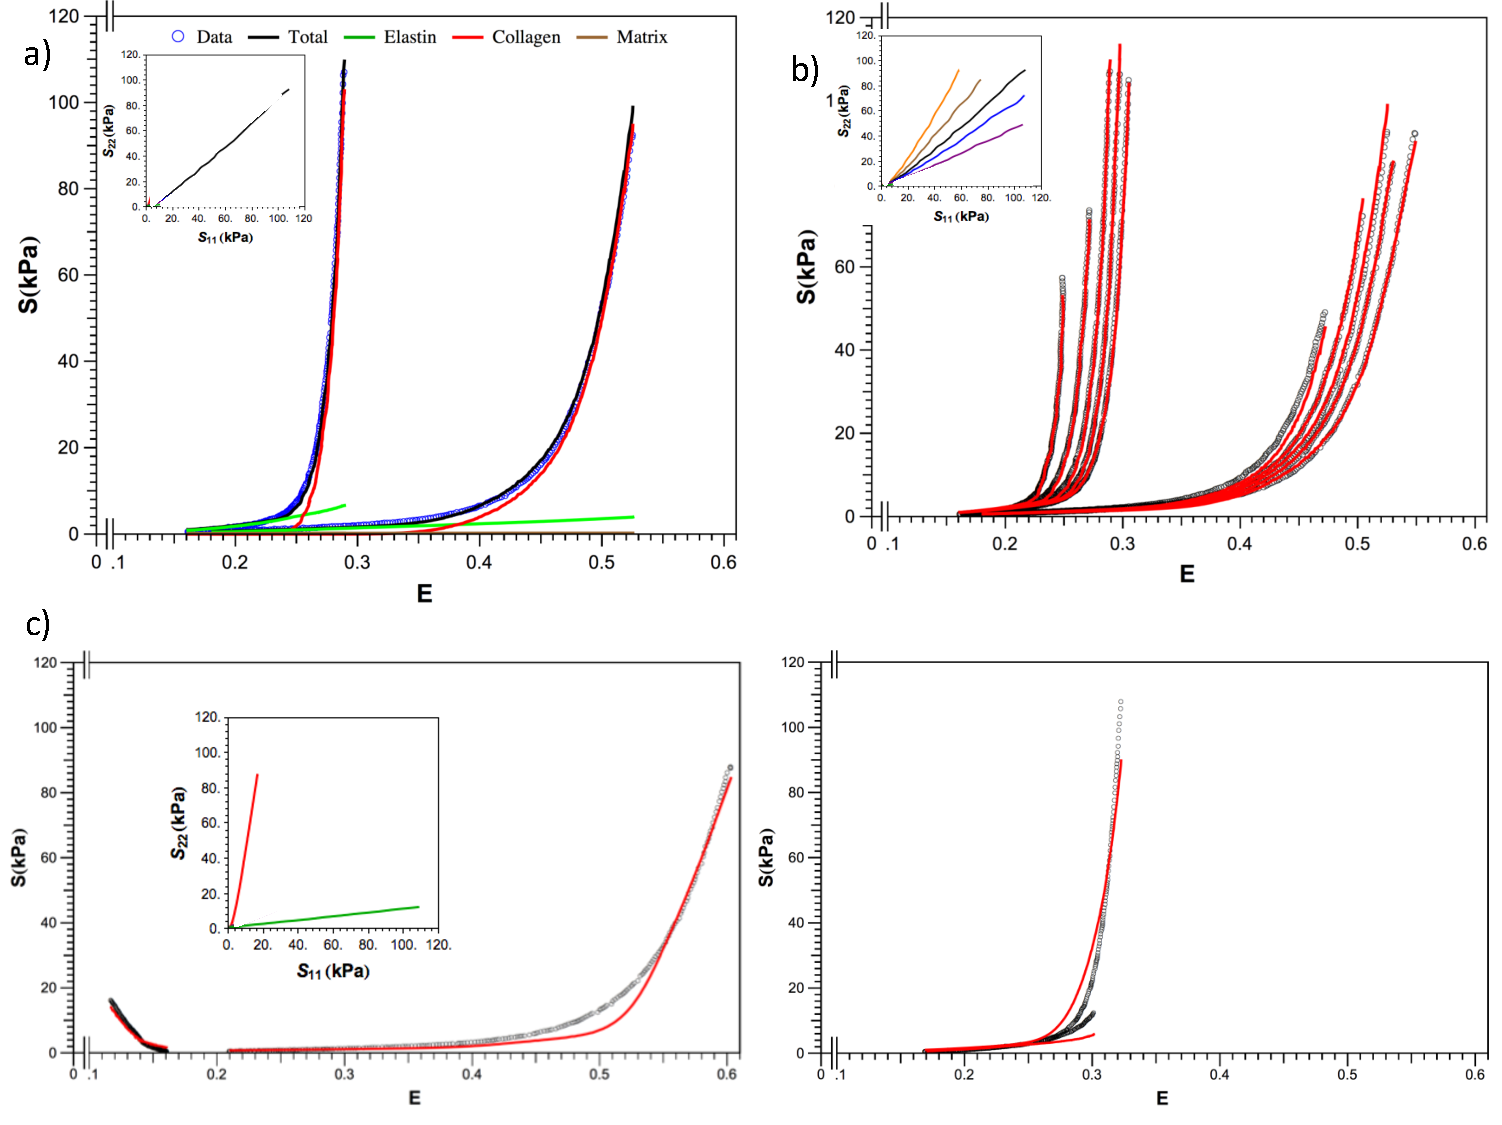
\includegraphics[width=\textwidth]{Images/chapter2/figure4.pdf}
\caption{Example of the best fit from an anterior leaflet. The (a) equibiaxial stress protocol was fit with only the elastin (green) first, followed by fitting the collagen only while keeping the elastin fixed. (b) The final fit of all “physiological” protocols are shown. (c) The two extra-physiological protocols, which were not fit, is show. This suggests that the model have good predictive capability.}
\label{c2:fig:4}
\end{figure}
%%%%%%%%%%%%%%%%%%%%	 end FIGURE 	%%%%%%%%%%%%%%%%%%%%




\subsubsection{Parameter estimation part 1 – collagen fiber recruitment} \label{c2:sec:2254}

    From the above analysis, the number of parameters was reduced to 22 (Table \ref{c2tab:modelparameters}). To start of the parameter estimation, we took advantage of the simplified kinematics of the uniaxial and EB test data to isolate the effects of collagen fiber recruitment in a simplified fiber recruitment model. For both datasets, the collagen fiber network in the fibrosa and ventricularis were idealized as a family of uni-directionally aligned fibers, with the elastin fibers neglected as their contributions to the total stress were insignificant in this loading state. Also note that for the EB tests the fiber ensemble stress can be determined directly by \cite{sacks_biaxial_2000}.
        %-------------------	begin EQUATION 	-------------------%
        \begin{equation}\label{c2eqn:ensembleform}
        \begin{aligned}
        S_{ens} = S_{11} + S_{22} \quad \text{for} \quad E_{11} = E_{22}, E_{12} = 0
        \end{aligned}
        \end{equation}
        %-------------------	 end EQUATION 	-------------------%
    We assumed in this first step that the recruitment distribution is orientation invariant, so that the collagen recruitment function $D(\mathbf{\xi},E_s) = D(\{\mu_r, \sigma_r, E_{lb}, E_{ub}\})$. $E_{ub}$ was determined by the transition point to the linear region (Fig. \ref{c2:fig:3}), leaving only $\mu r$, $\sigma r$ to be fit in this part of the parameter estimation. 
    
    
\subsubsection{Parameter estimation part 2 - full planar biaxial mechanical data set}

    Ideally, the measured ODFs $\Gamma(\theta)$ from the same specimen should be directly inserted into Eqn. \ref{eqn:multilayeredstressform}. However, in practice, we found that the ODFs had to be fitted to adjust for the specimen to specimen variability. Nevertheless, the mean best fitted ODFs can be compared to the mean measured ODFs to ensure that the estimate parameters are reasonable comparing to the true value. We expedited the process by assuming that the ODFs for each specimen is not significantly different from the true measured mean ODFs. Thus, the mean ODFs can be used as an initial guess and speed up the convergence to the optimal value. The use of a global algorithm will also ensure the optimized parameters do not become trapped at the mean value. Similarly, the estimated recruitment distribution $D(\mathbf{\xi}, x)$ is also obtain from independent specimens. The recruitment distribution parameters $\mathbf{\xi}$ are again used only as initial guesses and parameter validation.
    

    Taking a similar approach to Fata et al. \cite{fata_insights_2014}, we first examined the equibiaxial stress protocol ($P_{11}:P_{22}$ = 1:1), which is the best approximation of the in vivo loading state of the MV. The low stress region as defined in section \ref{c2:sec:elastinfibermodel} was used to fit the elastin (Fig. \ref{c2:fig:4}a). This is easily identified as the nearly linear response before the exponential like collagen response. Furthermore, due to limitations concerning the elastin model form, where the elastin response can increase exponentially to unrealistically surpass the response of the collagen, the exponent parameter d for the elastin (Table \ref{c2tab:modelparameters}) was constrained to be less than 3.5. Next, the remaining high stress region was used to fit the collagen fiber response independently. Using this coupled approach, we were able to minimize the search space to the 12 parameters associated with collagen (Table \ref{c2tab:modelparameters}). Once a reliable estimate of the parameters was obtained for this protocol, the inner 3 protocols (3:4, 1:1, 4:3) were fit using the existing parameters as the initial guess. We then progressed to the remaining “physiological” protocols (1:2, 3:4, 1:1, 4:3, 2:1) once again keeping the previous parameters as the initial guess to obtain better estimated parameters.
    
    
    Preliminary attempts demonstrated that gradient algorithms were unable to converge to the proper solution and tended to become unable to handle local minimas. As a result, we employed the genetics-based differential evolution algorithm to perform the optimization, similar to Fata et al. \cite{fata_insights_2014}. To narrow down the search space and guide the optimization, initial guess was derived from the above mechanical studies (Section \ref{c2:sec:mechanicalstudies}). Parameter estimation was performed using a custom program written in Mathematica (Wolfram Research Corp.).
    




\subsection{Model validation} \label{c2:sec:26}

    The mean fitted fiber ODFs $\Gamma(\theta)$ from each layer of the MV anterior leaflet were compared to the measured ODFs obtained from SHG imaging (section \ref{c2sec:structure}). Since the orientation of the fibers are referenced to the laboratory testing or imaging configurations for the mechanical and imaging data respectively, which may be different, the preferred direction of the $\Gamma(\theta)$ were rotated to $\mu_\theta = 0^\circ$ to give the appropriate comparison. Next, in the SAXS study \cite{liao_relation_2007}, the average fibril strain for all fibrils in the leaflet, $\bar{\epsilon}_\mathrm{fibril} = \bar{\lambda}_t - 1$, where  is the mean true stretch of the fibrils, was measured. Since the loading protocol was equibiaxial stress ($P_{11}$:$P_{22}$ = 1:1), the tissue was in an anisotropic strain state, with each fiber ensemble experience different ensemble strain. Additionally, the fiber slack strain reduces the effective stiffness of the fibrils at the tissue-level (Eqn. \ref{eqn:collagenfiberlaw}). Hence we needed to incorporate the $\Gamma_c(\theta)$ as well as collagen fiber recruitment distribution ($D(\mathbf{\xi}, x)$) in the SAXS simulations. The correct fiber modulus ($\eta$) is also necessary to determine the tissue-level stress. Therefore, SAXS gives us an independent method to validate the collagen network model used in this study.
    
    
    To simulate the full SAXS response, as compared to those measured by Liao et al. \cite{liao_relation_2007}, we assume standard affine kinematics (section \ref{sec:generalconsiderations}) \cite{lee_presence_2015}. Thus the fibril stretch is equal to the true stretch of the collagen fibers. Using structural parameters determined from parameter estimation, we simulated a population of fibers based on the fiber ODF and collagen recruitment distributions. The fibers were then deformed based on the EB tension protocol. This corresponds to a mean true fiber stretch given by
        %-------------------	begin EQUATION 	-------------------%
        \begin{equation}\label{c2:eqn:fibrilstrain}
        \begin{aligned}
        \bar{\lambda}_t = \int_\theta\Gamma(\theta)\left[\int_1^{\lambda_{ens}(\theta)}D(\mathbf{\xi},x)\frac{\lambda_{ens}(\theta)}{x}\dif x\right]\dif \theta
        \end{aligned}
        \end{equation}
        %-------------------	 end EQUATION 	-------------------%
    The resulting mean fibril strains $\bar{\epsilon}_\mathrm{fibril} = \bar{\lambda}_t-1$ were plotted against the measured tissue-level stresses and compared to the SAXS $\epsilon_\mathrm{fibril}$ \cite{liao_relation_2007}.


\subsection{Statistical testing}

    Standard independent two-sample t-tests were used to determine the statistical significance of the results.



    
    
    
    

%---    Results
\section{Results}

\subsection{Uniaxial and EB strain analysis} \label{c2:sec:uniaxialandEBresults}

    It was observed under these tests that the resulting stress–strain responses transitioned to a linear region prior to failure (Fig. \ref{c2:fig:3}). This observation supported the use of a collagen fiber recruitment model for MV tissue (Section \ref{sec:generalconsiderations}). Under EB strain testing kinematics, full recruitment was reached on average at a mean and standard deviation value of $0.284\pm0.047$ in Green’s strain and $782.1\pm121.5$ kPa in ensemble stress for the anterior leaflet. For the posterior leaflet, full recruitment strain was achieved at $0.2730\pm0.0156$ in Green strain and $1434.0\pm165.4$ kPa in ensemble stress. The posterior leaflet appeared to recruit more gradually than that of the anterior leaflet, with an average $\sigma_r$ (the standard deviation of the collagen fiber recruitment function) of $0.0231\pm0.001$ in Green strain compared to $0.015\pm0.003$ for the anterior leaflet. In comparison, the average maximum tensile strength under uniaxial loading along the circumferential direction for the anterior leaflet was 2, $220.1\pm794.5$ kPa. This suggests that the stress required to tear the tissue is approximately three times higher than the stress required to reach full recruitment on average.
    

\subsection{Parameter estimation}

    For the fitted parameters obtained from uniaxial extension and EB strain datasets (Section \ref{c2:sec:2254}, Table \ref{c2:tab:4}, Table \ref{c2:tab:5}), we observed similar collagen modulus $\eta_c$ for both tests. There appeared to be a shift in strain for the recruitment parameters values due to the differences in testing methodology. For all specimens tested under the full planar tension test protocols, they demonstrated a clear toe region at stresses below 7 kPa. This gave us a good initial estimate of the elastin response in comparison to the final fitted values, while fitting the high stress region resulted in recruitment parameter values that were consistent with EB strain testing (Fig. \ref{c2:fig:4}a). The fit of the full model (Eqn. \ref{eqn:multilayeredstressform}) (Fig. \ref{c2:fig:4}b) had a very good mean R-squared value of 0.964 for the anterior leaflet and 0.951 for the posterior leaflet (Table \ref{c2:tab:6}, Table \ref{c2:tab:7}). The full model (Eqn. \ref{eqn:multilayeredstressform}) was used to predict the stress of the extra-physiological protocols and obtained similar results (Fig. \ref{c2:fig:4}c and d). The modulus of the collagen fibers was found to be $164.0 \pm 16.4$ MPa for the anterior and posterior leaflets under planar tension, which is comparable for all mechanical data (Fig. \ref{c2:fig:5}a, Table \ref{c2:tab:4}, \ref{c2:tab:5}, \ref{c2:tab:6}, \ref{c2:tab:7}).
    
    
\begin{table}
\centering
\caption{Uniaxial extension testing results for the MV anterior leaflet.}\label{c2:tab:4}
\begin{tabular}{L{.5in}L{0.8in}L{0.6in}L{0.6in}L{0.6in}}
\hline
 & $\mathbf{\eta}_c \mathrm{(MPa)}$  & $\mu_r^f$ & $\sigma_r^f$ & $E_{ub}^f$  \\
\hline
1 & 68.2420 & 0.12543 & 0.01602 & 0.1434    \\
2 & 345.6285 & 0.23445 & 0.02099 & 0.2558   \\
3 & 114.5181 & 0.13822 & 0.02682 & 0.1592   \\
4 & 25.7835 & 0.11667 & 0.02545 & 0.1592    \\
\hline
Mean & 138.5431 & 0.15369 & 0.02232 & 0.1794    \\
SEM & 71.3667 & 0.02728 & 0.00244 & 0.0257      \\
\hline
\end{tabular}
\end{table}


\begin{table}
\centering
\caption{Equibiaxial strain testing results.}\label{c2:tab:5}
\begin{tabular}{L{.4in}L{.5in}L{.5in}L{.5in}L{.5in}L{.5in}L{.5in}L{.5in}L{.5in}}
\hline
 & \multicolumn{4}{l}{\textbf{Anterior}} & \multicolumn{4}{l}{\textbf{Posterior}}   \\
 \hline
 & $\mathbf{\eta}_c$  & $\mu_r^f$ & $\sigma_r^f$ & $E_{ub}^f$ 
 & $\mathbf{\eta}_c$  & $\mu_r^f$ & $\sigma_r^f$ & $E_{ub}^f$        \\
 \hline
1 & 83.93 & 0.270 & 0.023 & 0.298 & 151.06 & 0.200 & 0.022 & 0.224    \\
2 & 146.67 & 0.187 & 0.009 & 0.194 & 118.51 & 0.272 & 0.023 & 0.293   \\
3 & 218.24 & 0.178 & 0.008 & 0.184 & 149.48 & 0.260 & 0.024 & 0.287   \\
4 & 143.29 & 0.280 & 0.023 & 0.302 & 155.48 & 0.222 & 0.021 & 0.250   \\
5 & 188.67 & 0.427 & 0.013 & 0.442 & 127.20 & 0.283 & 0.026 & 0.311   \\
\hline
Mean & 156.16 & 0.268 & 0.015 & 0.284 & 140.34 & 0.247 & 0.023 & 0.273      \\
SEM & 22.78 & 0.045 & 0.003 & 0.047 & 7.338 & 0.016 & 0.0008 & 0.0156       \\
\hline
\end{tabular}
\end{table}


%%%%%%%%%%%%%%%%%%%%	begin FIGURE 	%%%%%%%%%%%%%%%%%%%%
\begin{figure}
\centering
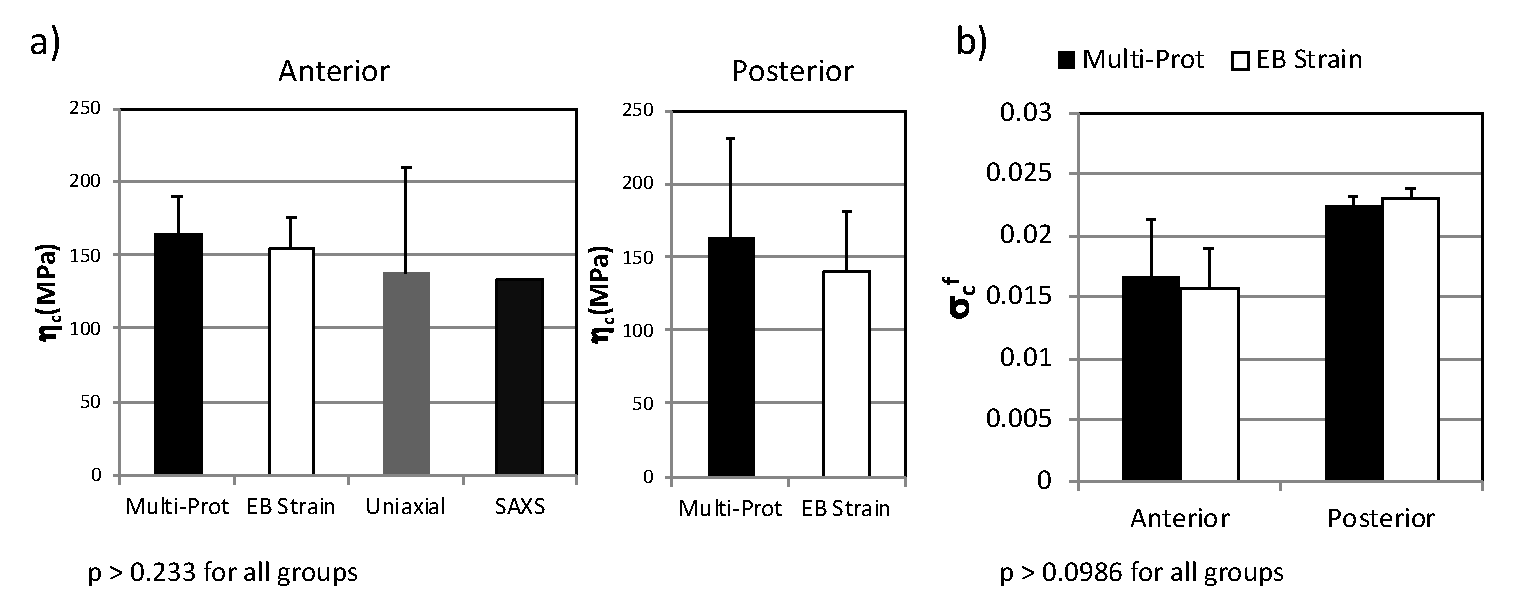
\includegraphics[width=\textwidth]{Images/chapter2/figure5.pdf}
\caption{(a) The mean and standard deviation of the collagen fiber modulus as determined from uniaxial, equibiaxial strain, and planar biaxial stress testing for both the anterior and posterior leaflets is shown. No statistical significant was found from ANOVA and student-t tests. (b) The mean and standard deviation of $\sigma_r$, which is standard deviation of the recruitment distribution of collagen fibers, in the fibrosa layer for both the anterior and posterior leaflet is shown. Again, no statistical significance was found, but the posterior leaflet appears to have larger $\sigma_r$ based on the trend.}
\label{c2:fig:5}
\end{figure}
%%%%%%%%%%%%%%%%%%%%	 end FIGURE 	%%%%%%%%%%%%%%%%%%%%


\begin{sidewaystable}
\centering
\caption{Parameter estimation results from the MV anterior leaflet.}\label{c2:tab:6}
\begin{tabular}{L{.5in}L{.55in}L{.4in}L{.4in}L{.4in}L{.4in}L{.4in}L{.4in}L{.4in}L{.4in}L{.4in}L{.4in}L{.4in}}
\hline
& \multicolumn{12}{c}{\textbf{Collagen}}    \\
\cline{2-13}
& \textbf{Modu.} & \multicolumn{4}{c}{\textbf{Fibrosa + Ventricularis}} & \multicolumn{4}{c}{\textbf{Atrialis}} & \multicolumn{3}{c}{\textbf{Spongiosa}}  \\
\hline
\textbf{ID} & $\mathbf{\eta}_c$ & $\sigma_c^f$ & $\mu_r^f$ & $\sigma_r^f$ & $E_{ub}^f$ & $\sigma_c^a$ & $\mu_r^a$ & $\sigma_r^a$ & $E_{ub}^a$ & $\mu_r^s$ & $\sigma_r^s$ & $E_{ub}^s$   \\
\hline
1 & 144.92 & 0.163 & 0.210 & 0.010 & 0.223 & 0.465 & 0.864 & 0.042 & 0.989 & 0.790 & 0.015 & 0.835  \\
2 & 86.23 & 0.140 & 0.522 & 0.010 & 0.537 & 0.077 & 1.172 & 0.019 & 1.204 & 1.177 & 0.038 & 1.256   \\
3 & 235.26 & 0.075 & 0.425 & 0.041 & 0.494 & 0.075 & 0.613 & 0.028 & 0.653 & 0.676 & 0.015 & 0.720  \\
4 & 199.33 & 0.136 & 0.293 & 0.011 & 0.307 & 0.075 & 0.914 & 0.010 & 0.927 & 0.890 & 0.010 & 0.902  \\
5 & 207.55 & 0.149 & 0.391 & 0.006 & 0.397 & 0.400 & 1.791 & 0.154 & 2.099 & 1.798 & 0.006 & 1.810  \\
6 & 196.41 & 0.180 & 0.286 & 0.015 & 0.307 & 0.250 & 0.520 & 0.019 & 0.545 & 0.525 & 0.015 & 0.559  \\
7 & 69.35 & 0.222 & 0.275 & 0.024 & 0.300 & 0.075 & 0.472 & 0.015 & 0.517 & 0.540 & 0.026 & 0.617   \\
Mean & 162.72 & 0.153 & 0.335 & 0.017 & 0.361 & 0.170 & 0.759 & 0.022 & 0.806 & 0.766 & 0.020 & 0.815   \\
SEM & 26.16 & 0.020 & 0.047 & 0.005 & 0.051 & 0.066 & 0.111 & 0.005 & 0.113 & 0.100 & 0.004 & 0.103 \\


\hline
& \multicolumn{8}{c}{\textbf{Elastin}} & & \textbf{Mat.} & \textbf{Ori.} & \textbf{$R^2$}  \\
\cline{2-13}
& \multicolumn{3}{c}{\textbf{Ventricularis}} & \multicolumn{3}{c}{\textbf{Atrialis}} & \multicolumn{2}{c}{\textbf{Spongiosa}} & & & &  \\
\hline
\textbf{ID} & $\mathbf{\eta}_e^v$ & $d^v$ & $\sigma_e^v$ & $\mathbf{\eta}_e^v$ & $d^v$ & $\sigma_e^v$ & $\mathbf{\eta}_e^v$ & $d^v$ & & $\mathbf{\eta}_m$ & $\mu_\theta$ &    \\
\hline
1 & 53.91 & 2.878 & 0.077 & 125.0 & 1.732 & 0.078 & 54.67 & 2.747 & & 0.000 & 0.304 & 0.980   \\
2 & 0.07 & 3.416 & 0.079 & 0.12 & 2.982 & 0.082 & 0.04 & 1.742 & & 0.010 & 0.350 & 0.893      \\
3 & 12.25 & 3.500 & 0.077 & 27.21 & 3.000 & 0.079 & 0.06 & 2.986 & & 0.000 & 0.622 & 0.957    \\
4 & 14.52 & 3.000 & 0.076 & 67.28 & 1.000 & 0.151 & 0.00 & 2.048 & & 0.000 & 0.384 & 0.986    \\
5 & 2.08 & 2.980 & 0.106 & 0.05 & 1.681 & 0.340 & 0.00 & 1.553 & & 0.911 & -0.05 & 0.970     \\
6 & 13.71 & 3.443 & 0.081 & 287.3 & 2.132 & 0.097 & 0.00 & 2.824 & & 0.281 & 0.449 & 0.996    \\
7 & 2.33 & 1.886 & 0.199 & 0.34 & 2.704 & 0.341 & 0.00 & 3.000 & & 0.000 & -0.20 & 0.970     \\
Mean & 16.13 & 3.021 & 0.098 & 84.55 & 2.258 & 0.138 & 9.13 & 2.558 & & 0.049 & 0.274 & 0.964 \\
SEM & 7.9 & 0.250 & 0.020 & 44.94 & 0.324 & 0.042 & 9.13 & 0.217 & & 0.047 & 0.102 & 0.015    \\
\hline
\end{tabular}
\end{sidewaystable}



\begin{sidewaystable}
\centering
\caption{Parameter estimation results from the MV Posterior leaflet.}\label{c2:tab:7}
\begin{tabular}{L{.5in}L{.55in}L{.4in}L{.4in}L{.4in}L{.4in}L{.4in}L{.4in}L{.4in}L{.4in}L{.4in}L{.4in}L{.4in}}
\hline
& \multicolumn{12}{c}{\textbf{Collagen}}    \\
\cline{2-13}
& \textbf{Modu.} & \multicolumn{4}{c}{\textbf{Fibrosa + Ventricularis}} & \multicolumn{4}{c}{\textbf{Atrialis}} & \multicolumn{3}{c}{\textbf{Spongiosa}}  \\
\hline
\textbf{ID} & $\mathbf{\eta}_c$ & $\sigma_c^f$ & $\mu_r^f$ & $\sigma_r^f$ & $E_{ub}^f$ & $\sigma_c^a$ & $\mu_r^a$ & $\sigma_r^a$ & $E_{ub}^a$ & $\mu_r^s$ & $\sigma_r^s$ & $E_{ub}^s$   \\
\hline
1 & 200.000 & 0.352 & 0.300 & 0.011 & 0.314 & 0.400 & 0.487 & 0.033 & 0.539 & 1.554 & 0.168 & 2.020 \\
2 & 197.276 & 0.247 & 0.393 & 0.010 & 0.411 & 0.400 & 0.840 & 0.051 & 0.966 & 1.911 & 0.157 & 2.218 \\
3 & 96.535 & 0.422 & 0.715 & 0.044 & 0.760 & 0.427 & 2.500 & 0.158 & 2.966 & 1.329 & 0.020 & 1.369  \\
4 & 160.354 & 0.216 & 0.543 & 0.010 & 0.558 & 0.400 & 1.323 & 0.052 & 1.436 & 2.028 & 0.018 & 2.079 \\
5 & 200.000 & 0.370 & 0.454 & 0.033 & 0.501 & 0.104 & 1.366 & 0.048 & 1.480 & 0.780 & 0.037 & 0.824 \\
6 & 181.100 & 0.292 & 0.608 & 0.017 & 0.639 & 0.400 & 1.380 & 0.079 & 1.563 & 1.079 & 0.039 & 1.196 \\
7 & 112.588 & 0.325 & 0.392 & 0.032 & 0.428 & 0.400 & 0.699 & 0.064 & 0.890 & 1.668 & 0.107 & 1.811 \\
Mean & 163.979 & 0.318 & 0.486 & 0.022 & 0.516 & 0.362 & 1.228 & 0.069 & 1.406 & 1.478 & 0.078 & 1.645  \\
SEM & 16.330 & 0.027 & 0.054 & 0.005 & 0.057 & 0.043 & 0.251 & 0.016 & 0.296 & 0.169 & 0.025 & 0.197    \\



\hline
& \multicolumn{8}{c}{\textbf{Elastin}} & & \textbf{Mat.} & \textbf{Ori.} & \textbf{$R^2$}  \\
\cline{2-13}
& \multicolumn{3}{c}{\textbf{Ventricularis}} & \multicolumn{3}{c}{\textbf{Atrialis}} & \multicolumn{2}{c}{\textbf{Spongiosa}} & & & &  \\
\hline
\textbf{ID} & $\mathbf{\eta}_e^v$ & $d^v$ & $\sigma_e^v$ & $\mathbf{\eta}_e^v$ & $d^v$ & $\sigma_e^v$ & $\mathbf{\eta}_e^v$ & $d^v$ & & $\mathbf{\eta}_m$ & $\mu_\theta$ &    \\
\hline
1 & 83.48 & 2.866 & 0.129 & 789.7 & 1.686 & 0.400 & 234.7 & 2.610 & & 0.001 & -0.60 & 0.993  \\
2 & 1.537 & 2.705 & 0.082 & 0.029 & 3.000 & 0.085 & 0.011 & 1.000 & & 0.000 & -0.04 & 0.967  \\
3 & 0.743 & 2.918 & 0.349 & 0.000 & 2.999 & 0.400 & 0.000 & 2.549 & & 0.000 & -0.31 & 0.864  \\
4 & 0.685 & 2.884 & 0.078 & 1.223 & 1.006 & 0.092 & 0.041 & 2.874 & & 0.000 & 1.425 & 0.930   \\
5 & 0.198 & 1.044 & 0.285 & 2.993 & 2.116 & 0.393 & 0.778 & 3.000 & & 0.426 & -0.39 & 0.972  \\
6 & 0.103 & 1.001 & 0.075 & 0.000 & 2.731 & 0.311 & 0.000 & 1.774 & & 0.253 & -0.23 & 0.984  \\
7 & 1.789 & 2.050 & 0.285 & 239.3 & 3.000 & 0.400 & 119.7 & 3.000 & & 0.333 & -0.16 & 0.985  \\
Mean & 12.65 & 2.210 & 0.183 & 147.6 & 2.363 & 0.297 & 50.74 & 2.401 & & 0.145 & -0.32 & 0.956   \\
SEM & 11.81 & 0.326 & 0.045 & 112.2 & 0.297 & 0.055 & 34.98 & 0.283 & & 0.071 & 0.170 & 0.017 \\
\hline
\end{tabular}
\end{sidewaystable}


    Next, we compared the result for the two collagen fiber recruitment models: orientation-invariant (Eqn. \ref{eqn:recruitmentasafunctionnormal}) and orientation-variant (Eqn. \ref{eqn:recruitmentasafunctionofangle}). Interestingly, we found no major difference between these modeling approaches (Fig. \ref{c2:fig:6}). The R-squared value of fit was very good for both models ($R^2$ = 0.996 vs 0.988 for Eqns. \ref{eqn:recruitmentasafunctionnormal}, \ref{eqn:recruitmentasafunctionofangle} respectively). There were no significant difference in the predicted collagen fiber modulus $\eta_c$ (Fig. \ref{c2:fig:6}a) and the collagen fiber $\Gamma(\theta)$ shows only a difference of $0.44^\circ$ in $\eta_c$ for the atrialis and $1.21^\circ$ in  for the fibrosa (Fig. \ref{c2:fig:6}b). Furthermore, the collagen fiber recruitment distribution $D(\mathbf{\xi}, x)$ when scaled to the same range [0,1] by their upper-bound value (Fig. \ref{c2:fig:6}c) were similar for either case.
    
    
%%%%%%%%%%%%%%%%%%%%	begin FIGURE 	%%%%%%%%%%%%%%%%%%%%
\begin{figure}
\centering
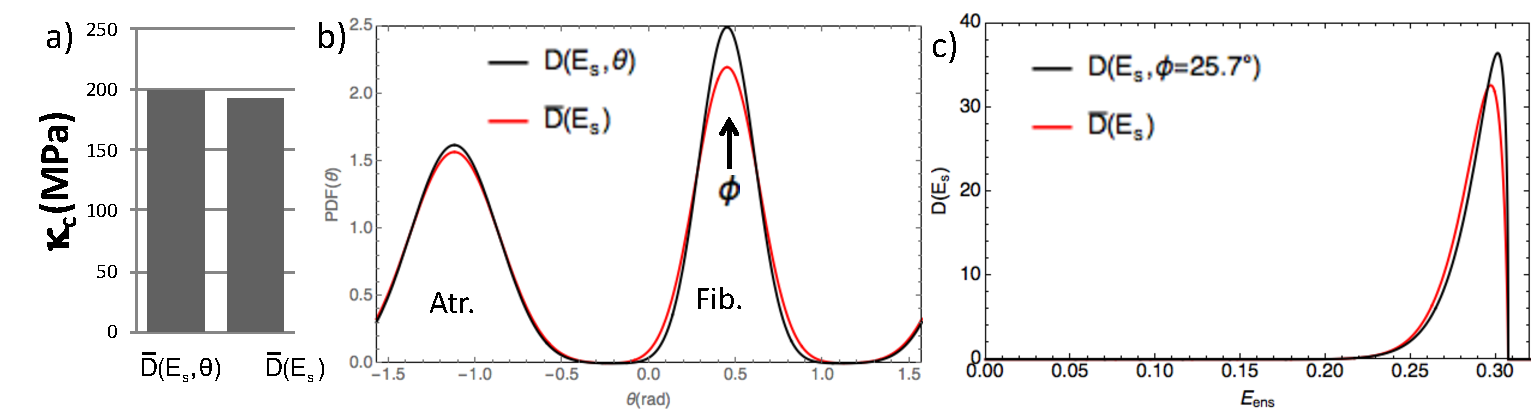
\includegraphics[width=\textwidth]{Images/chapter2/figure6.pdf}
\caption{The specimen was fit using both the comparisons for the orientation-variant $\bar{D}(\bar{\mathbf{\xi}},x)$ (Black) and orientation invariant $D(\mathbf{\xi},x,\mathbf{n}_0)$ (Red) modeling approaches for the recruitment functions. Both methods produce (a) nearly the same collagen fiber modulus. (b) The fiber ODFs also appears to the equivalent width ($\sigma_c^f$). (c) The recruitment distribution also appears to be similar.}
\label{c2:fig:6}
\end{figure}
%%%%%%%%%%%%%%%%%%%%	 end FIGURE 	%%%%%%%%%%%%%%%%%%%%
    
    
    The optimal recruitment parameters for both the multi-protocol data and the EB strain data were very similar (Table \ref{c2:tab:5}, \ref{c2:tab:6}, \ref{c2:tab:7}). We found no significant differences in the averaged standard deviation of recruitment, $\sigma_r$, between the anterior and posterior leaflets for either tests (Fig. \ref{c2:fig:5}b). There were minor differences in the distributions due to the way the upper-bound parameter was determined. The analysis of the EB strain kinematic state was done visually, where the upper-bound may have been underestimated. For analysis of the stress controlled planar biaxial tests, which does not reach full recruitment, the upper-bound was predicted by the parameter estimation algorithm and tended to be slightly overestimated. Uniaxial testing instead shows a very different recruitment response (Table \ref{c2:tab:4}). This is most likely due to the vastly different testing modes, where the differences in preconditioning and gauge length result in a drastically different reference state for the fibers. Additionally, fiber rotation effects in the uniaxial testing slow the recruitment of fibers away from the test axis and produce a greater standard deviation for the recruitment distribution. We however observe in trend that the posterior leaflet recruits slower than the anterior leaflet (Fig. \ref{c2:fig:5}b), possibly due to differences in their role mechanically during valve closure.
    
    


\subsection{Parameter validation} \label{c2:sec:233}

    Perhaps the most important validation finding was that the simulated SAXS response (Eqn. \ref{c2:eqn:fibrilstrain}), using the best fit parameters, matched very well to the MV SAXS data from Liao et al. \cite{liao_relation_2007} (Fig. \ref{c2:fig:7}). The squared correlation coefficient was computed ($r^2 = 0.971$), and we found no statistical significance ($p = 0.285$) between the two curves. To assess the sensitivity of the SAXS simulation (Eqn. \ref{c2:eqn:fibrilstrain}), the origin recruitment distribution parameters $\mu_r^f = 0.286$ and $E_{ub}^f = 0.307 $ were shifted by $\pm0.01$ in Green Lagrange strain, and the standard deviation of the collagen fiber ODF $\sigma_r^f = 10.3^\circ (\Gamma_c(\theta))$ was adjusted by $\pm1^\circ$ (Fig. \ref{c2:fig:7}). Despite the perturbation being so small, there was a 54\% increase in the slope of the simulated SAXS response when the mean and upper-bound of the recruitment was increased by 0.01, and a 38\% decrease in slope when the parameters were decreased by 0.01. Similarly, the slope decreased by 17\% when  was increased by $1^\circ$, and increased by 20\% when decreased by $1^\circ$. 
    An estimate of the fiber modulus for the MV SAXS data was made by comparing against the simulated data. No statistical significance for the collagen fiber modulus between any mechanical tests or between either leaflets was found. In addition, the predicted ODFs $\Gamma_c(\theta)$ and $\Gamma_e(\theta)$ compared very well with the SHG measurements, with standard deviations differing by no more than 3 degrees (Fig. \ref{c2:fig:8}). Thus, despite the model complexity, these validation results suggest that the parameters were sufficiently independent and each can be accurately determined as a representation of the mechanical behavior of the MV.
    
    
%%%%%%%%%%%%%%%%%%%%	begin FIGURE 	%%%%%%%%%%%%%%%%%%%%
\begin{figure}
\centering
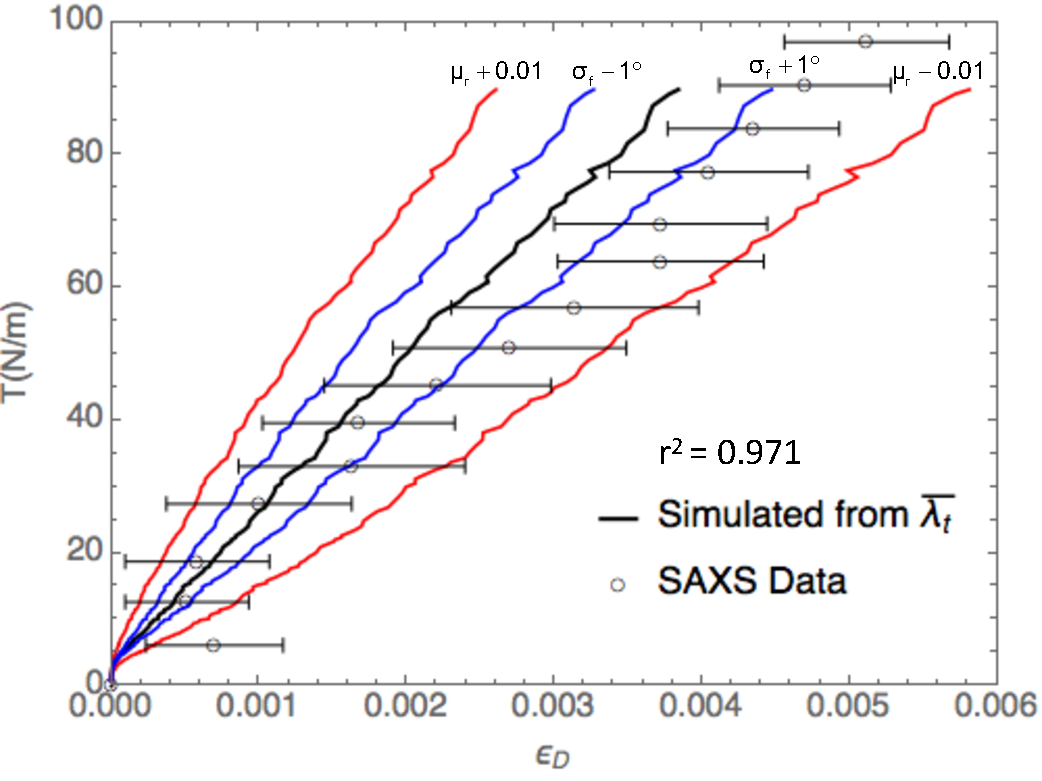
\includegraphics[width=0.75\textwidth]{Images/chapter2/figure7.pdf}
\caption{Collagen fibril stress–strain data from SAXS studies from Liao et al. \cite{liao_relation_2007} (circles) along with the simulated result based on the current model parameters (Black) showing very good agreement. This approach is very sensitive. Perturbing the ODF ($\sigma_c^f$) by $1^\circ$ (Blue) and shifting the recruitment distribution by 0.01 in Green strain (Red) significantly changed the slop of the curve.}
\label{c2:fig:7}
\end{figure}
%%%%%%%%%%%%%%%%%%%%	 end FIGURE 	%%%%%%%%%%%%%%%%%%%%


%%%%%%%%%%%%%%%%%%%%	begin FIGURE 	%%%%%%%%%%%%%%%%%%%%
\begin{figure}
\centering
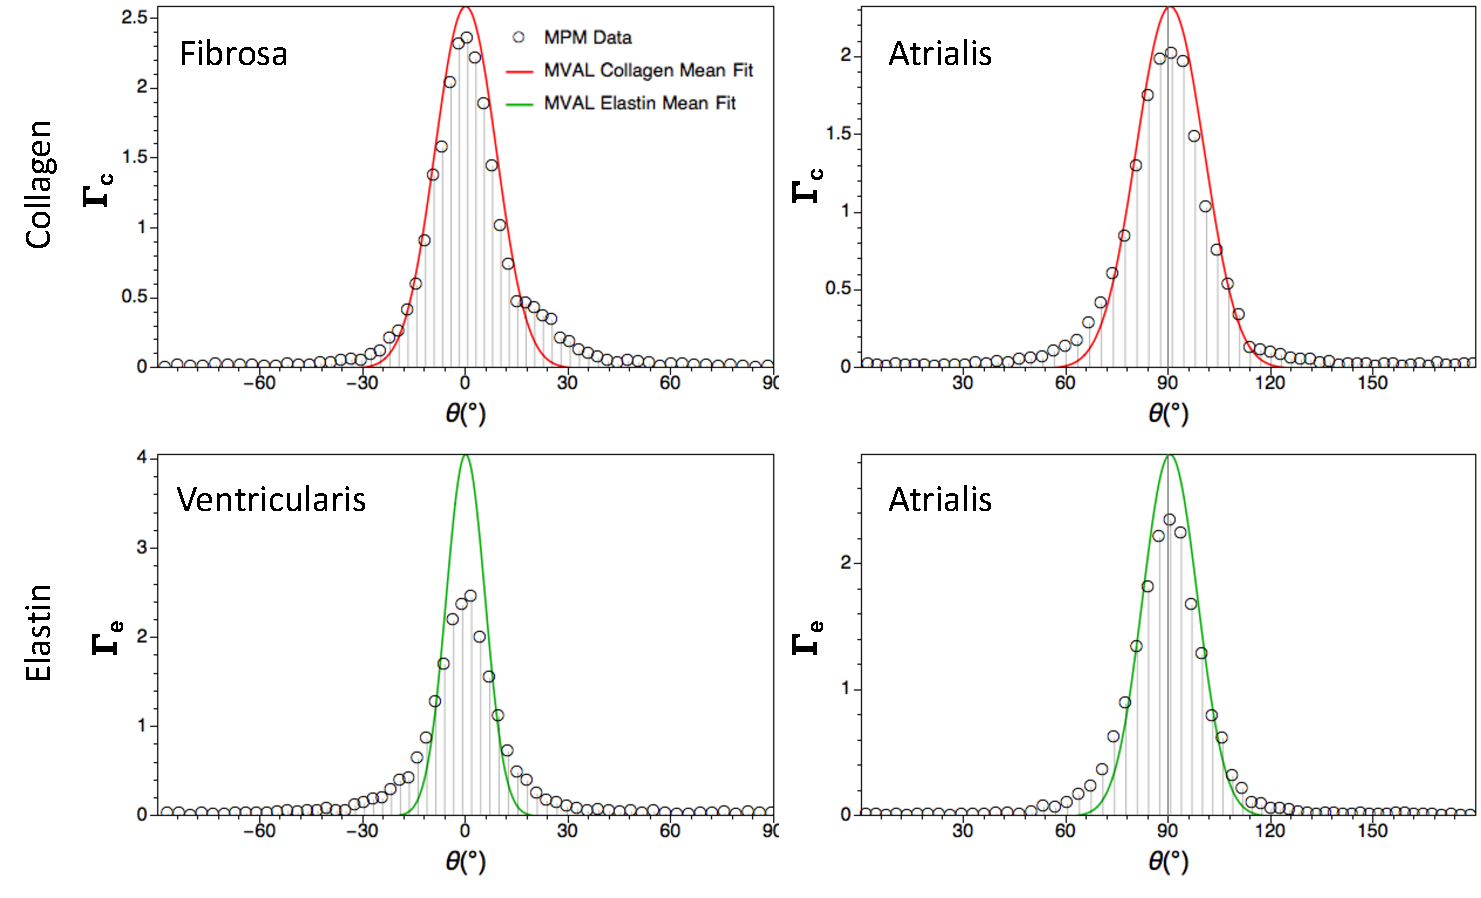
\includegraphics[width=\textwidth]{Images/chapter2/figure8.pdf}
\caption{The fitted orientation distribution functions of the collagen (Red) and elastin (Green) for the anterior leaflet are shown in comparison to the measured distribution from SHG (circle). The results are shown for the ventricularis, fibrosa and atrialis. The fitted and measured ODF appears to show good agreement. }
\label{c2:fig:8}
\end{figure}
%%%%%%%%%%%%%%%%%%%%	 end FIGURE 	%%%%%%%%%%%%%%%%%%%%




\subsection{Differences between layers and leaflets}

    All ODFs $\Gamma(\theta)$ of the ventricularis, fibrosa and atrialis were much narrower in the anterior leaflets than the posterior leaflets (Fig. \ref{c2:fig:9}). To estimate the mean ensemble elastin response, each elastin ensemble was scaled by the principle strain at maximum loading under EB stress and then averaged. Like the structural differences between the anterior and posterior leaflets, the mechanical response of ventricularis was much stiffer in the anterior leaflets comparing to the posterior leaflet (Fig. \ref{c2:fig:10}). On the other hand, the atrialis was stiffer in the posterior leaflet (Fig. \ref{c2:fig:10}). For the overall layer contributions, the mechanical response of the circumferential direction is mainly due to the elastin in the ventricularis at lower stress and the collagen within the fibrosa at high stress, whereas the radial direction is a combination of collagen fibers in the fibrosa as they extend and rotate under physiological loading and collagen in the atrialis at higher strains (Fig. \ref{c2:fig:11}). The mechanical contribution from the spongiosa was, as anticipated, negligible for both leaflets.
    
    
%%%%%%%%%%%%%%%%%%%%	begin FIGURE 	%%%%%%%%%%%%%%%%%%%%
\begin{figure}
\centering
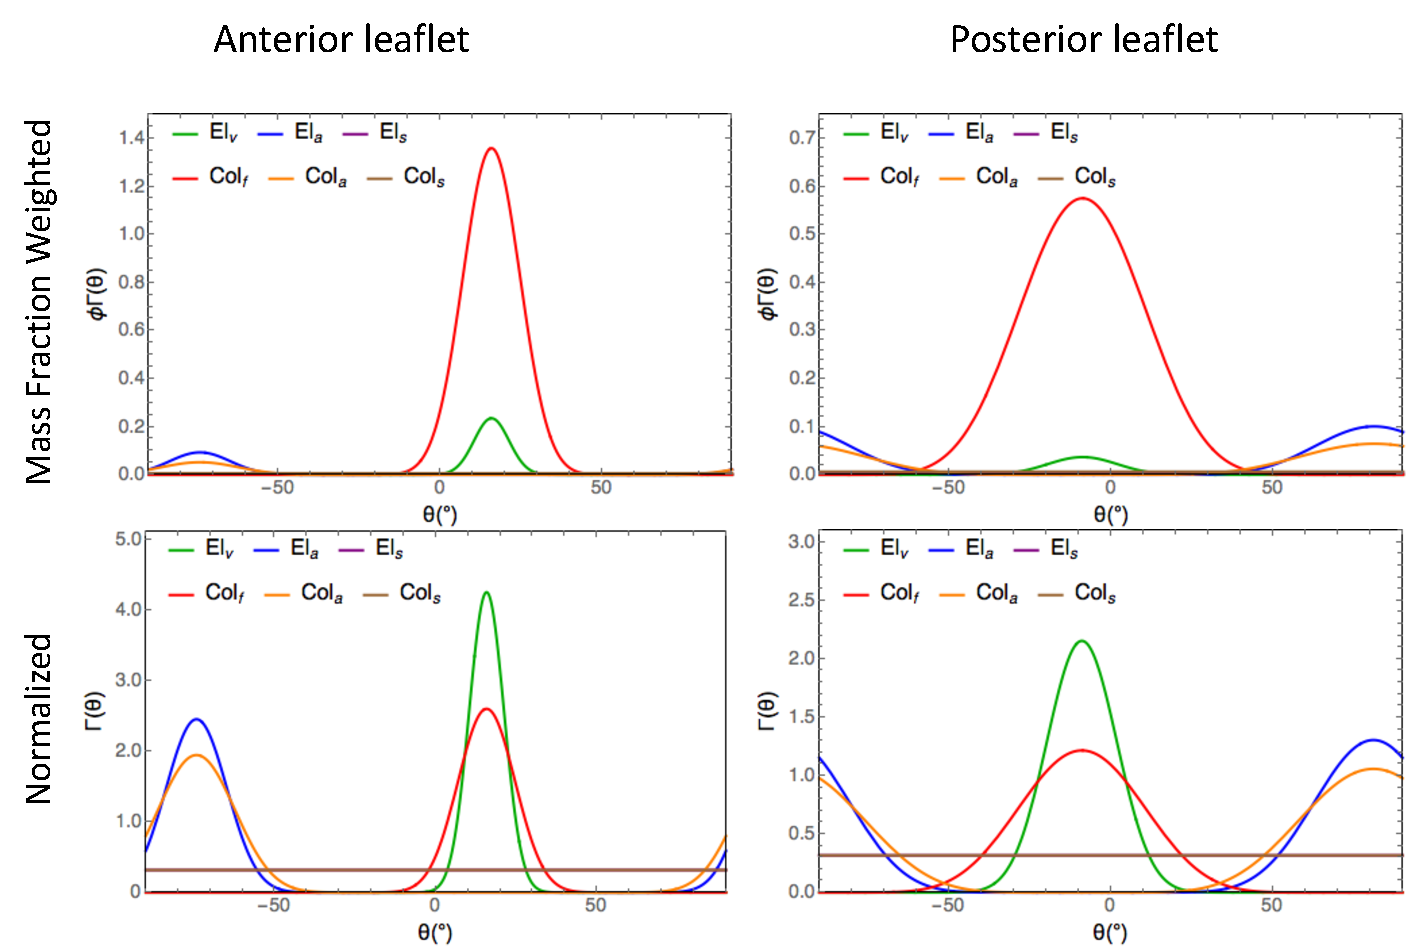
\includegraphics[width=\textwidth]{Images/chapter2/figure9.pdf}
\caption{The predicted fiber orientation distributions from the anterior (Left) and posterior leaflets (Right) for collagen and elastin from all layers as an average (n = 7 for both leaflets). Both the mass fraction scaled (Top) and normalized (Both) ODFs are shown. In both leaflets the collagen of the fibrosa layer is clearly the most dominant, but is more broadly distributed in the posterior leaflet. Elastin is also similarly trends but is more evenly distributed in the anterior leaflet, while favoring the atrialis in the posterior leaflet.}
\label{c2:fig:9}
\end{figure}
%%%%%%%%%%%%%%%%%%%%	 end FIGURE 	%%%%%%%%%%%%%%%%%%%%


%%%%%%%%%%%%%%%%%%%%	begin FIGURE 	%%%%%%%%%%%%%%%%%%%%
\begin{figure}
\centering
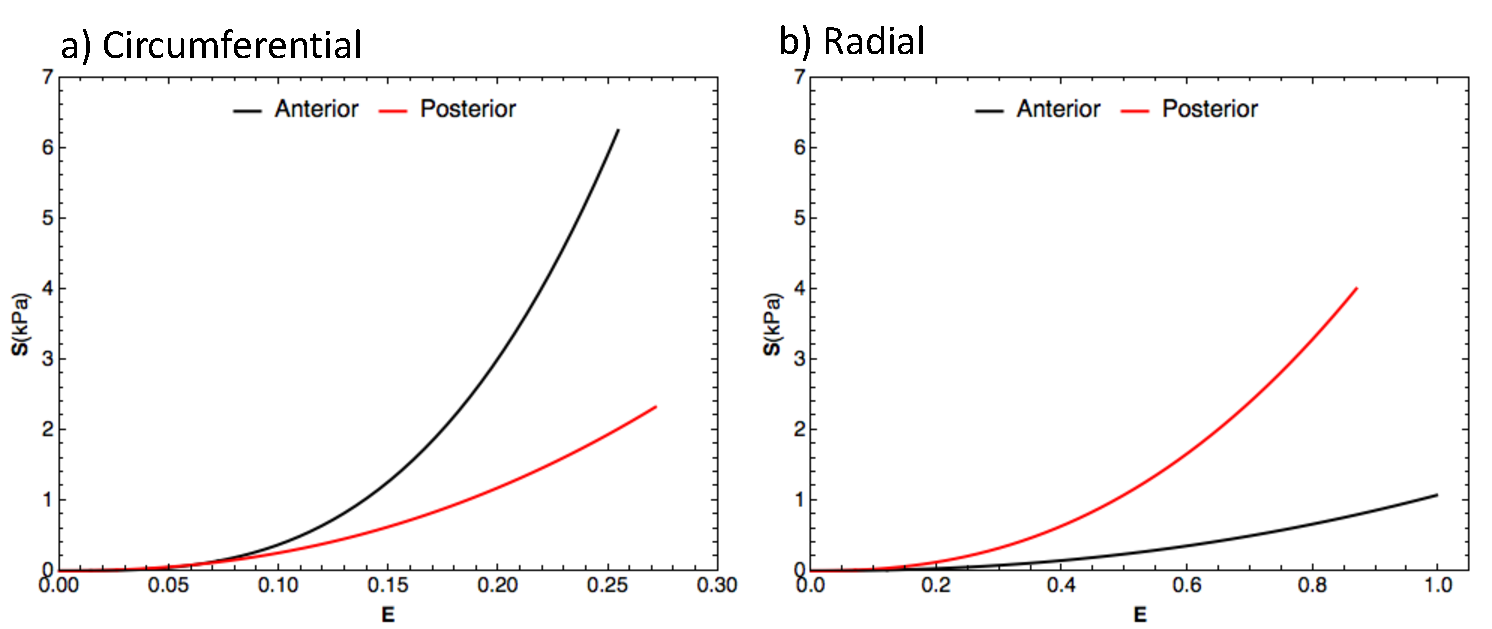
\includegraphics[width=\textwidth]{Images/chapter2/figure10.pdf}
\caption{The mean elastin response in the physiological range from both anterior (Black) and posterior (Red) leaflets in the circumferential (a) and radial (b) directions. n = 7 for both leaflets. The elastin in the anterior leaflet is heavily anisotropy and favoring the circumferential direction, which the elastin in the posterior leaflet is more isotropic and only slightly favoring the radial direction.}
\label{c2:fig:10}
\end{figure}
%%%%%%%%%%%%%%%%%%%%	 end FIGURE 	%%%%%%%%%%%%%%%%%%%%


%%%%%%%%%%%%%%%%%%%%	begin FIGURE 	%%%%%%%%%%%%%%%%%%%%
\begin{figure}
\centering
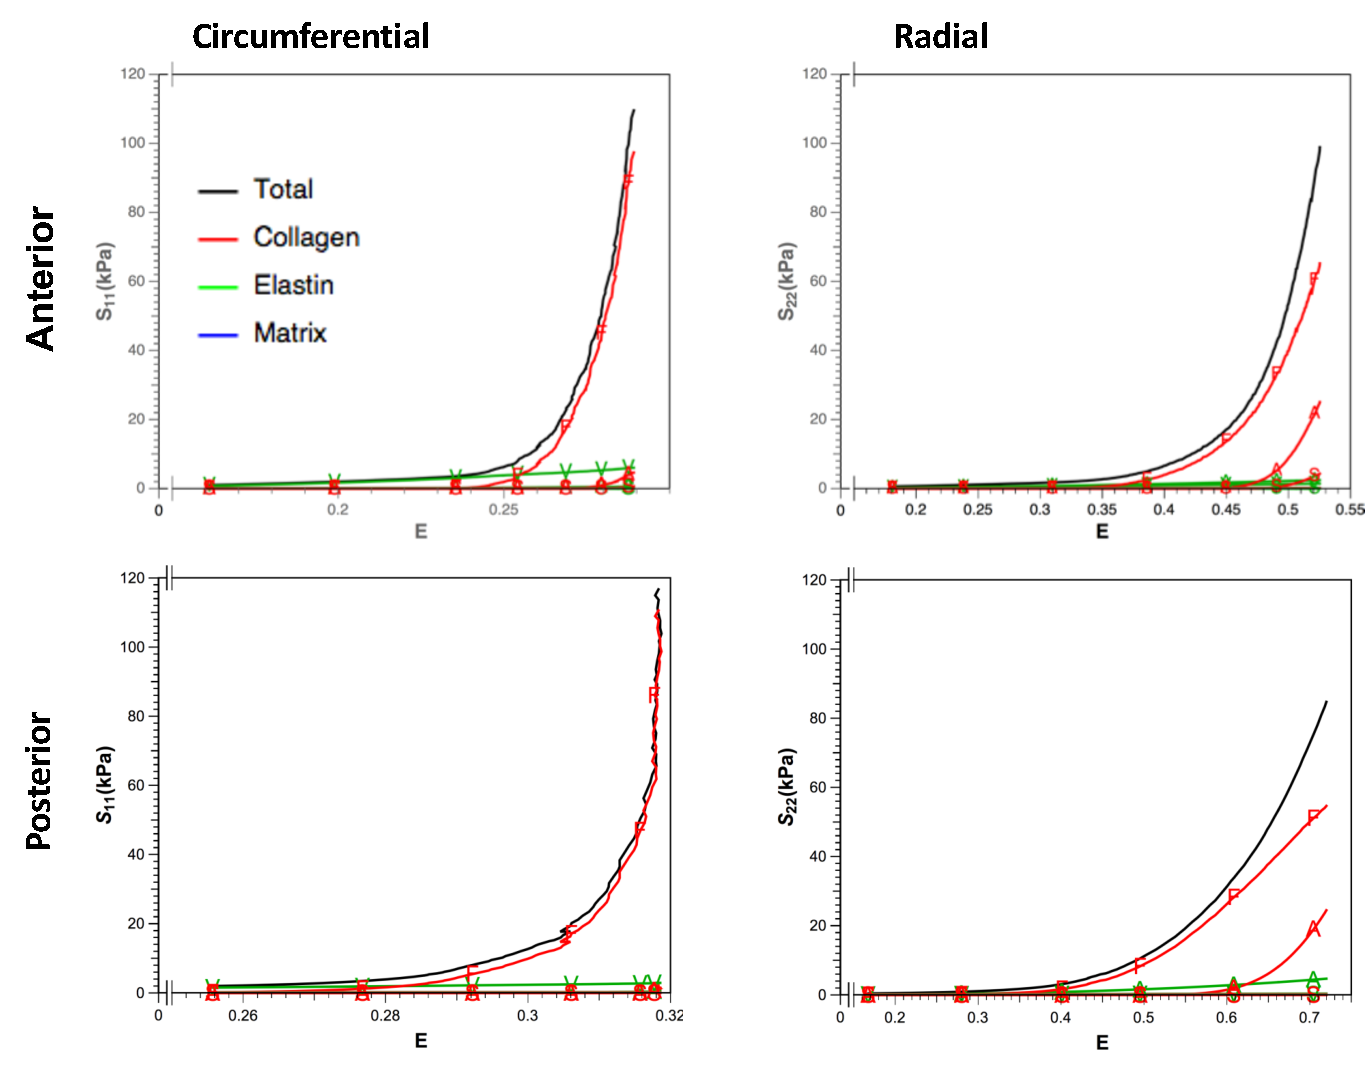
\includegraphics[width=\textwidth]{Images/chapter2/figure11.pdf}
\caption{The net stress contribution from each ECM component from each layer for the equibiaxial stress protocol is shown for the circumferential (Left) and radial (Right) direction of the anterior (Top) and posterior (Bottom) leaflets. Here, the contributions from the layers are ventricularis (V), fibrosa (F), spongiosa (S), and atrialis (A). Interestingly, while the fibrosa layer is dominant circumferential directions in both leaflets, the atrialis also contributes substantially in the radial direction. Elastin clearly contributes minimal stress comparing to collagen, but it forms the bulk of the response in the toe region.}
\label{c2:fig:11}
\end{figure}
%%%%%%%%%%%%%%%%%%%%	 end FIGURE 	%%%%%%%%%%%%%%%%%%%%






%---    Discussion
\section{Discussion}

\subsection{Modeling approach and major findings}

    In the present study, we developed a novel layer-specific meso-scale structural model of the MV leaflets starting from the fiber-level. The mechanical response at the layer- and tissue-level is driven by structural measurements and observations obtained from SHG and histology. We then utilized an extensive experimental mechanical database that included uniaxial, planar EB strain, and a comprehensive set planar biaxial stress test protocols. This approach allowed us to properly evaluate the mechanical properties of MV tissues and to form a complete dataset for parameter estimation. All information was then integrated to form a predictive model for the MV leaflet tissues.
    
    
\subsection{Model validation}

    Novel to this study was the use of the MV SAXS data \cite{liao_relation_2007} to validate the predicted collagen fiber modulus and fiber recruitment (Section \ref{c2:sec:26}). SALS techniques have been previously used to obtain the orientation of fibrous structures in biological tissues \cite{sacks_small_1997}. However, the wavelength of light (in the hundreds of nm) is much too large in comparison the size of the fibrils, which have a D-period of approximately 64 nm \cite{kastelic_structural_1980,hodge_recent_1963,chapman_electron_1984}. SAXS, on the other hand, utilizes a wavelength of 0.1–0.2 nm, and provides a direct way of measuring the collagen fibril D-period, and thus the fibril strains \cite{sasaki_elongation_1996,sasaki_stress_1996,liao_relation_2007}. In response to tissue-level deformation, the fibril strain depends on both its orientation and slack strain (Section \ref{c2:sec:26}). Therefore, the MV SAXS simulation can provide an independent way of validating the MSSCM collagen model component. Both the good agreement and sensitivity to accurate measures (Section \ref{c2:sec:233}, Fig. \ref{c2:fig:7}) provides additional confidence in our approach beyond basic measures such as goodness of fit. In particular, this lends confidence to the fiber/fibril kinematics used in the present form of the MSSCM, and suggests that the fibrils do indeed form contiguous, tightly bounded fibers and undergo minimal slipping.
    
    
    It is also important to note that it is difficult to directly combine measurements at multiple scales, such as fibril strain as measured by SAXS and the applied tissue-level membrane stress, and interpret them directly. In this case, we cannot approximate the modulus of collagen fibrils using the slope of the tissue-level stress–fibril strain curve. Although we assume every fibril has a similar modulus, the apparent modulus of collagen fibrils at the tissue-level decreases in response to increase in the slack stretch (Eqn. \ref{eqn:collagenfiberlaw}). Thus interpretation of such results requires careful analysis of the structure and kinematically related mechanisms of the tissue. Finally, we also validated the fiber $\Gamma(\theta)$ against optical SHG measurements, which demonstrated very good agreement (Fig. \ref{c2:fig:8}). To the authors’ knowledge, this is the first time macro/micro validations of this kind have been performed for any soft tissue
    
    


\subsection{Collagen fiber modulus}

    As the most important load bearing component of soft tissues, the structure and properties of collagen is of major interest. One specific property is the modulus of the collagen fiber, which when combined with the level of fiber undulation, determines the macroscopic behavior of the collagen network at the tissue-level. Given that type I collagen fibers forms the common building blocks for the bulk of the MV tissue (Fig. \ref{c2:fig:2}), the modulus serves both as an important validation for the results of the model and predicting the correct behavior of the tissue under complex loading conditions. There have been many attempts to measure the stiffness of collagen fibers in the literature \cite{shen_stress_2008,gentleman_mechanical_2003,eppell_nano_2006,yang_mechanical_2008,yang_micromechanical_2007,wenger_mechanical_2007}. These measurements come in two forms: (1) models at the tissue-level and (2) direct measurements at the fibril-level. Measurements at the tissue-level can be inaccurate, as they demand an extensive understanding of biomechanics of the tissue, physically accurate models of the mechanical behavior and detailed measurements of the structure and composition. On the other hand, there is currently no method for the real time estimation of the instantaneous cross sectional area of collagen fiber or fibrils. Current measurements are typically done a priori \cite{gentleman_mechanical_2003} or a posteriori \cite{eppell_nano_2006}, and can have significant impact on the results. These measurements also require highly accurate and noise insensitive instruments operating at the micrometer and nanometer scale. As such, these experiments are typically done using techniques such as atomic force microscopy (AFM) and have a large variability for the resulting numbers. Nonetheless, these measurements serve as an important reference for any results measure at the tissue-level, and the current literature paints a distinct picture.


    For the most part, these findings fall into two distinct categories: (1) the dried properties at the 2–10 GPa range and (2) hydrated properties at the 200–900 MPa range. This difference in stiffness is due to water acting as a plasticizer in collagen fibrils [62]. Using AFM, Yang et al. \cite{yang_micromechanical_2007} found a stiffness of 1.4 GPa for non-cross linked fibrils and 3.4 GPa for cross-linked collagen fibrils in the bovine Achilles tendon. Similarly, Wenger et al. \cite{wenger_mechanical_2007} found collagen fibril stiffness of 5–11.5 GPa in rat tail tendon. However, in both papers the fibrils were dried under ambient conditions and nitrogen, respectively. On the other side, Shen et al. \cite{shen_stress_2008} found a modulus of $860\pm450$ MPa for collagen fibrils obtained from sea cucumber dermis. In the study by Gentleman et al. [23], they found a modulus of $269.7\pm11.9$ to $484.7\pm76.3$ MPa for collagen fibers in the bovine Achilles tendon, varying with the fiber diameter, but only for the cross-linked fibers. Eppell et al. \cite{eppell_nano_2006}, found a modulus of 0.5–0.4 GPa at low strain (0.05–0.30) but can increase to up to 12 GPa at high strain. In these cases, the fibrils were hydrated before testing. This effect has also been studied using electrospun collagen scaffolds, where Yang et al. found that the fibril modulus decrease from 1.3–7.8 GPa to 0.07–0.26 GPa when hydrated\cite{yang_mechanical_2008}.


    In present study we found the collagen fiber modulus to be between 132.5 and 167.3 MPa. In our estimation of the collagen volume fraction, we assumed the tissue is entirely composed of collagen, elastin and proteoglycans. While this serves as a good estimation of the relative composition of the MV, fluid constitutes 81.8\% of the total mass of the MV anterior leaflet \cite{lis_biochemical_1987}. Additionally, using the dry mass is not a viable alternative as the fibers may have shrunk when they are dried \cite{leikin_raman_1997}. As such, we chose the current approach to provide an unbiased effective collagen modulus for the MV. This value is not applicable to other tissues with significantly different structural composition and may explain minor differences in the modulus estimate for the anterior and posterior leaflet. When the residual volume is taken into account, it is not difficult to imagine the estimated modulus to be 2–4 times higher than the value reported, allowing it to fall in line with the modulus of the hydrated collagen fibrils in other studies. This suggests that the model is reasonably accurate in estimating the mechanical properties of the collagen fibers. Furthermore, there were no statistical significance between the fiber modulus for either leaflet, which is reasonable given that the majority of collagen fibers are type I. Finally, that the assumption of minimal fiber–fiber and fiber–matrix interaction appears to be essentially correct. This is consistent with the ability for the fibers to rotate and extend freely with applied forces, keeping the effective tissue modulus low so the leaflets can coapt as necessary for valve function.
    
    
    
    
\subsection{Collagen fiber recruitment}

    While type I collagen naturally occurs in a crimped state, the bending stiffness as the collagen fiber unravels is typically small enough to allow us to use the recruitment approach \cite{lanir_constitutive_1983,fata_insights_2014,sacks_incorporation_2003,lanir_structural_1979,kastelic_structural_1980,hansen_recruitment_2002,cacho_constitutive_2007,grytz_constitutive_2009}. Novel to recruitment approach, we propose an angle variant recruitment distribution based on the hypothesis that the ensemble stress will be limited to a small range due to homeostasis. Current experimental techniques do not easily allow for direct measurement, and distinguishing individual fibers is difficult and sometimes required to be specified manually \cite{hill_theoretical_2012}. Determining whether a fiber is straightened is also problematic. For best accuracy, the fiber must lay in the plane of the image. The planar projection of a fiber at an angle with the plane of the image creates a misrepresentation of the tortuosity of the fiber. Additionally, the tissue must be loaded under EB strain with no shearing. Failure to do so will result in different strain for each fiber ensemble, thus the tortuosity of fibers at different angle cannot be referenced to the same strain. These issues are further magnified when quantifying angular variations. In the end, direct measurement methods are best served as a preliminary estimate for modeling purposes.


    Assuming that the ensemble stress of collagen fibers is constant with orientation due to homeostasis, both the current model (Eqn. \ref{eqn:recruitmentasafunctionofangle}) and the orientation-variant model (Eqn. \ref{eqn:recruitmentasafunctionnormal}) produce similar results for the MV leaflets; the quality of the best fits ($R^2 = 0.988$ vs $0.996$) are very comparable for both models. We hypothesize that this is due to the narrow splay of the collagen fiber ODF in the MV and thus the ensemble stress was effectively constant over this range for both models. This simplifies the recruitment distribution function for implementation in MV simulation and measurement via experimental means. Also, by assuming orientation-variance in Eqn. \ref{eqn:recruitmentasafunctionofangle}, the parameters are expressed as a percentage of the maximum ensemble strain, which is not an intuitive quantity. Thus, the parameters determined from Eqn. \ref{eqn:recruitmentasafunctionofangle} are best served as an approximation, rather than any physically accurate quantity. Therefore, we refocused the results as if the recruitment strains are invariant with angle (Eqn. \ref{eqn:recruitmentasafunctionnormal}), which has a more interpretive physical meaning. In either case, the theory then dictates that the tissue should exhibit a linear response once all fibers are straightened under EB strain loading. Indeed, this is observed in the MV for both the anterior (Fig. \ref{c2:fig:3}) and posterior leaflet.


    For each leaflet tested under EB strain and uniaxial extension, the stress strain curve transitions to linear in P–F \cite{sasaki_elongation_1996,sasaki_stress_1996,liao_relation_2007}. For the anterior leaflet this transition point occurs at $782.1\pm121.5$ kPa in 2nd Piola Kirchhoff or $1243.8\pm220.8$ kPa in Cauchy stress. Our inverse model using a full collagen mapped transverse model shows that the peak circumferential stress is at $241.4\pm40.5$ kPa and the peak radial stress is at $432.6\pm46.5$ kPa \cite{lee_inverse_2014}. While it is not possible to produce the equivalent ensemble stress for the in vivo data, it is estimated that only 20–40\% of fibers are recruited under physiological stress. This substantial structural reserve is likely an adaption to maintain structural integrity for when the body is under extraneous physiological stress or attempt to maintain basic function in cases of heart diseases.
    



\subsection{Elastin fiber network response}

    There is no established constitutive model form for individual elastin fibers in valvular tissue. We have taken a similar approach to modeling the fiber ensembles in the ovine pulmonary arteries \cite{fata_insights_2014}. However, in the MV, we noticed a slight nonlinearity in the pre collagen fiber recruitment response contrary to that of the pulmonary arteries \cite{fata_insights_2014}. It is not clear what the reason behind this is. Likely the cross-linking, both between and within a fiber in the elastin network, is different in order to fulfill the different functions for each tissue. To fit the low stress region, an exponential or power law is necessary. We chose the power law so we can constrain the order of the nonlinearity. This may result in some error when predicting and extrapolating past the range of the data. However, the stress contribution of elastin peaks at around 5–15 kPa at maximum stretch, which is much less that of the collagen (Fig. \ref{c2:fig:4}a), so this should not be a significant effect. The collagen also essentially functions as a stopper, putting a constraint on the maximum extension of the leaflets (especially in the circumferential direction). For this reason, the material model of the elastin this should not be a problem for the predictive capabilities of the model in most applications.


    Another interesting result is that the exponents of the elastin model differed between the layers and between the leaflets. This may be evidence of residual stress or strain between the layers. For the aortic valve, Stella and Sacks \cite{stella_biaxial_2007} noted that the elastin dominant ventricularis of the leaflet contracted by 10.9\% and 8.2\% in the radial and circumferential direction while the collagen dominant fibrosa elongated by 28.2\% and 4.8\% in the radial and circumferential direction after layer separation. Similar effect likely exists in the MV and the additional strain will result in a higher apparent stiffness due to the nonlinearity in the stress strain response. Thus the difference in the atrialis and ventricular of each leaflet may, at least in part, be due to this reason. It is interesting that the elastin in the anterior leaflet is significantly stiffer in the circumferential direction compared to that of the posterior leaflet, while in the radial direction it was the opposite. This corroborates with physical observations where the ventricularis in the posterior leaflet was much smaller compared to the anterior leaflet; sometimes nearly nonexistent. Again, this may be a product of the motion of the leaflets when closing.
    
    
    
    
\subsection{Layer structure and function}

    In the MV, the anterior leaflet extends to meet the posterior leaflet, while the posterior expands much less in comparison \cite{amini_vivo_2012,rausch_vivo_2011}. In order to accomplish this, the radial direction of the anterior leaflet needs to be able to extend significantly, while the circumferential direction needs to be able to maintain its integrity as it meets the posterior leaflet. There are a number of ways in which collagenous tissue have adapted to increase extensibility. The most common way is through adjustment in the crimping of the collagen fibers. However, once fiber recruitment is initiated, the tangent modulus increases rapidly, limiting further extension. A second method is through the rotation of fiber ensembles. As the ratio of radial to circumferential stretch increases, this induces a rotation of all fibers toward the radial direction. The overall effect is similar to recruitment due to crimping, but the tangent modulus increases more gradually in comparison. Intriguingly, this adaptation is seen in the MV leaflets. For both leaflets, collagen is mostly present in the fibrosa (Fig. \ref{c2:fig:2}). This results in the majority of collagen fibers being circumferentially aligned. Rather than having independent family of fibers each dictating the mechanical response of each direction, this is highly coupled (Fig. \ref{c2:fig:11}), with the bulk of the stress in the radial direction coming from the circumferential splay. However, the collagen fibers in atrialis are still needed for additional support. This makes the width of the fibers splay dictate the resulting response. In the anterior leaflet, the elastin and collagen fiber splays are narrower (Fig. \ref{c2:fig:9}), thus increasing the radial extensibility. Comparatively, the wider splay in the posterior leaflet produce a slightly more isotropic response resulting in smaller radial extension. Additionally, collagen fibers are also recruited faster in the anterior leaflet to further constrain the circumferential extension. Overall, collagen primarily functions to limit extension, whereas elastin determines the motion of the valve in the low stress region. This is perhaps why the radial direction of the anterior leaflet has the lowest stiffness, which allows for the fastest rate of extension. Interestingly, elastin is also the stiffest in circumferential direction of the anterior leaflet, following a similar trend as the collagen. The elastin in the posterior leaflet is likewise more isotropic than that of the anterior.
    
    
    
    
\subsection{Model predictive capabilities}

    Overall the model demonstrated very good ability to predict the extraphysiological protocols (Fig. \ref{c2:fig:4}c \& d). Using the correct mass fractions, for the ratio of collagen in the fibrosa vs the atrialis in particular, was especially important for accurately predicting these extra-physiological protocols. For predictive purposes, more leeway can be given for the mass fraction of elastin. Since the layers are treated completely independent of each other (not sharing a single modulus), errors in the mass fraction is absorbed by the modulus.
    
    
    
    
\subsection{Limitations}

    While every effort was made to ensure tissue viability, all studies were performed under in vitro conditions. While there appears to be differences between the in vivo properties of MV anterior leaflet \cite{krishnamurthy_material_2008} and the passive properties measured in an in vitro setting \cite{grashow_planar_2006,may-newman_biaxial_1995}. The mechanism behind these estimated differences remain unknown. It is unlikely to be due to the contractile forces exerted by the MV interstitial cells on the surrounding ECM, which appears to be small \cite{buchanan_interlayer_2013}. Residual stress may be involved, as studies have shown that the MV leaflets are also under significant residual strain \cite{amini_vivo_2012}. Additionally, the viscoelastic properties of the MV were not considered in this model, however we have found that the leaflet tissues are essentially functionally elastic \cite{grashow_biaxial_2006,grashow_planar_2006}. Direct validation of the individual layer stress contributions is not currently available, as it requires the separation of the individual layers, which in itself is a complex task. Additionally, a more sophisticated model is also necessary to take into account the effect of residual strain on the mechanical response. Nevertheless, we have shown that our models have good predictive capabilities for the mechanical response and fiber orientations distributions, and are validated using SAXS studies. Overall, this model is a faithful representation of the structural function relationship of MV tissues.

%---    Conclusion
\section{Conclusions and future directions}

In this study, we developed a novel fiber- and layer-specific structurally-driven constitutive model of the MV leaflets. The model incorporated fiber ODFs for collagen and elastin, collagen fiber recruitment, and related fiber-level mechanical phenomena. The model was validated by simulating the SAXS experiments and compared against the measured response. The results were consistent and show that the model correctly predicted the collagen fibril deformations measured by SAXS. Furthermore, the material parameters estimated were also consistent under EB strain testing and uniaxial testing. Thus the model is validated both via microscopic and meso-scale measurement. For the MV leaflets, we determined an effective modulus of 132.5–167.3 MPa for the collagen fibers which matches well with existing literature. This result suggests the tissue structure is an important predictor of leaflet function, where the fiber ODF and recruitment couples to determine the mechanical response of each leaflet. Moreover, fiber ODF tends to be narrower and the recruitment tends to happen over a smaller strain range to allow for a larger extension of the anterior leaflets while maintaining tensile strength. Overall, the model shows very good predictive ability and hopes to help in producing more accurate simulations of MV behavior in vivo, with the ultimate goal in improving long-term durability of MV repair.

This model may also serve as a baseline for the study of disease and aging valvular tissues. Pathological change to biological tissue is a very complex topic. In addition to the variety of pathological conditions, the changes due to a common disorder will be different among individuals. There is not yet sufficient data to fully understand and predict the mechanical changes. However, this model can serve as a starting point for analyzing the underlying changes due to pathological conditions, when the requisite data become available.

We should note that the utility of the present model lies in the accuracy and details of how the various aspects of the MV tissue coordinate to produce the bulk-level response. This is not only important to ECM mechanics but also coupling to the interstitial cell (MVIC) population. We have recently shown that simulated MVIC moduli for the four layers were found to be all within a narrow range of 4.71–5.35 kPa, suggesting that MVIC deformation is primarily controlled by each tissue layer’s respective structure and mechanical behavior rather than the intrinsic MVIC stiffness \cite{lee_effects_2015}. This novel result further suggests that while the MVICs may be phenotypically similar throughout the leaflet, they experience layer-specific mechanical stimulatory inputs due to distinct extracellular matrix architecture and mechanical behaviors of the four MV leaflet tissue layers. This also suggests that MVICs may behave in a layer-specific manner in response to mechanical stimuli in both normal and surgically modified MVs. Development of detailed layer-specific models, such as the one presented herein, will clearly aid in further our understanding of these phenomena. However, for computational implementation, a multi-scale approach \cite{lee_mitral_2014} will likely be needed to make the current implementation computationally tractable.






\bibliographystyle{plainnat}
\bibliography{phd}





